\documentclass[10pt,reqno]{amsart} %This is the AMS article style, with default font size 10pt.
\usepackage{amssymb,alltt}
\usepackage[cp1250]{inputenc}   %podpora za sumnike
\usepackage{hyperref}
\usepackage[all]{xy}            %za diagrame risat: \xymatrix{}
\usepackage{tikz}
    \usetikzlibrary{shadows,matrix,arrows}
    \newcommand*\ccircled[1]{\tikz[baseline=(C.base)]\node[draw,rectangle,rounded corners,inner sep=1.9pt,line width=0.15mm](C){\normalsize#1};\!} %obkrozen tekst s krogom
\usepackage{mathtools}
\usepackage{longtable}

%\newtheorem{Stm}{statement}[section]
\newtheorem{Thm}[subsection]{Theorem}
\newtheorem{Prp}[subsection]{Proposition}
\newtheorem{Lmm}[subsection]{Lemma}
\newtheorem{Crl}[subsection]{Corollary}
\newtheorem{Cnj}[subsection]{Conjecture}
%The following gives definition type environments (which only differ from theorem type in the choices of fonts).  The numbering is tied to the theorem counter.
%\theoremstyle{definition}
%\newtheorem{Dfn}[Stm]{Definition}
%\newtheorem{Exp}[Stm]{Example}
%The following gives remark type environments (which only differ from theorem type in the choices of fonts). The numbering is tied to the theorem counter.
%\theoremstyle{remark}
%\newtheorem{Rmk}[Stm]{Remarks}
\numberwithin{equation}{section}

\def\id{\mathrm{id}}        %identity morphism
\def\opp{\mathrm{op}}       %opposite ring
\def\Ker{\mathrm{Ker}}
\def\Im{\mathrm{Im}}
\def\Hom{\mathrm{Hom}}
\def\Ext{\mathrm{Ext}}
\def\Tor{\mathrm{Tor}}
\def\N{\mathbb{N}}
\def\Z{\mathbb{Z}}
\def\Q{\mathbb{Q}}

\newcommand{\rd}[1]{\textcolor[rgb]{1.00,0.00,0.00}{#1}}
\newcommand{\gn}[1]{\textcolor[rgb]{0.00,1.00,0.00}{#1}}
\newcommand{\bl}[1]{\textcolor[rgb]{0.00,0.00,1.00}{#1}}
\newcommand{\gr}[1]{\textcolor[rgb]{0.6,0.6,0.6}{#1}}
\newcommand{\mns}{\!\raisebox{-0.5pt}{\scalebox{0.5}[1.0]{\( - \)}}\!}

\begin{document}
\title[Chain complex reduction using steepness matchings]{Chain complex reduction\\ using steepness matchings}
\author{Leon Lampret}
\address{Faculty of Mathematics and Physics, Department of Mathematics, University of Ljubljana, Slovenia}
\email{lampretl@gmail.com, leon.lampret@fmf.uni-lj.si}
\date{March 2, 2019}
\keywords{algebraic/discrete Morse theory, homological algebra, chain complex, acyclic matching, algebraic combinatorics, algorithm implementation, \textsc{Mathematica}, code}
\subjclass{17B56, 13P20, 13D02, 55-04, 18G35, 58E05}
%\urladdr{www.math.sc.edu/$\sim$howard}


\begin{abstract}
Computing the homology of a chain complex with algebraic Morse theory is like doing Gaussian elimination, but only \emph{on certain columns/rows} and \emph{with several pivots} (in all the matrices at once). This significantly reduces fill-in and coefficient growth of the matrices, but it requires the construction of the set of pivots (called a Morse matching).
\par On any chain complex of free modules of finite rank, we define a family of acyclic matchings in the context of AMT. These pairings 
%enable a parallelized/multicore computation of homology. Most importantly, they 
have relatively small memory requirements. The downside is that applying such a matching gives a (significantly smaller) homotopy-equivalent chain complex, but not necessarily its homology directly (except when working over a field or a local PID).
\par Many acyclic matchings in the literature are special instances of this construction. In fact, we show that \emph{every} acyclic matching is a \emph{subset} of some matching from our family, so all maximal Morse matchings are of this type.
\par We provide \textsc{Mathematica} code for this reduction and compare its performance with \textsc{SageMath} algorithms. Using it, we computed (on a laptop) the homology (over $\Z_2$ and $\Q$, with generators) of a chain complex of Heisenberg Lie algebras, where the largest matrix is bigger than 20 million $\times$ 20 million.
\end{abstract}

\maketitle
%\tableofcontents

\subsection*{Motivation} Since chain complexes have become an important part of many mathematical areas, there is a big demand for efficient methods (with regard to the processor as well as the memory load) for the computation of their homology. Unfortunately, this continues to be a hard problem, since it appears it is still infeasible to compute with sparse matrices $\partial_k$ larger than $10^6\!\times\!10^6$. 
\par Note that in general, \textit{the bigger the matrices in $C_\ast$ get, the sparser they become}. For instance, in the Poincar\'{e} / Eilenberg-MacLane / Hochschild / Chevalley chain complex, the $k$-th matrix has density: 
\begin{itemize} \setlength{\itemindent}{-8mm}
	\item $=\frac{k\cdot f_k}{f_{k\!-\!1}\cdot f_k}\xrightarrow{f_{k\!-\!1}\to\infty}0$, where $f_k$ is the number of $k$-faces of the simplicial complex;
	\item $=\frac{(k+1)\cdot n^k}{n^{k\!-\!1}\cdot n^k}\xrightarrow{n\to\infty}0$, where $n$ is the cardinality of the group;
	\item $<\frac{(k+1)n\cdot n^{k+1}}{n^k\cdot n^{k+1}}\xrightarrow{n\to\infty}0$, where $n$ is the dimension of the associative algebra;
	\item $<\frac{\binom{k}{2}n\cdot \binom{n}{k}}{\binom{n}{k\!-\!1}\cdot \binom{n}{k}}\xrightarrow{n\to\infty}0$, where $n$ is the dimension of the Lie algebra.
\end{itemize}
Therefore, it makes sense to concentrate on methods that work best on sparse chain complexes, so we assume the matrices contain mainly zeros.
\par I offer a new algorithm, which reduces the size of all boundary matrices $\partial_k$ at once, by deleting every row $i$ and column $j$ that contain an invertible entry $\partial_{k,i,j}$ which has zeros left and below it (i.e. $\partial_{k,i,<j}\!=\!0\!=\!\partial_{k,>i,j}$), and (possibly) alters the remaining entries. The capabilities of my implementation are documented in \ref{performance}. It requires no computation of the Smith normal forms or ranks of matrices.

\subsection*{Conventions} Throughout this article, $R$ will be a commutative unital ring and\vspace{-1mm} \[C_\ast\!: C_0\!\overset{\partial_1}{\leftarrow}\!C_1\!\leftarrow\!\ldots\!\leftarrow\!C_{N\!-\!1}\!\overset{\partial_N}{\leftarrow}\!C_N\vspace{-1mm}\] a chain complex of free  $R$-modules of finite rank. Also, $R^\times$ is the group of units (=invertible elements) of $R$, e.g. $\Z^\times\!=\!\{1,-1\}$ and $K^\times\!=\!K\!\setminus\!\{0\}$ for any field $K$. %In all boundary matrices, only the nonzero entries will be displayed.
\vspace{4mm}

\section{Introduction to AMT}
\noindent My algorithm uses algebraic Morse theory, so I include a concise review of it. 
\subsection{Formulation} Pick a basis $I_k$ for each $C_k$. Let $\Gamma_{\!C_\ast}$ be a graph, with vertex set the disjoint union $\bigsqcup_kI_k$, and for every nonzero matrix entry $\partial_{k,u,v}\!=\!w \in R\!\setminus\!\{0\}$ a directed weighted edge $u\!\overset{w}{\leftarrow}\!v$. 
\par A \emph{Morse matching} is any collection $\mathcal{M}$ of edges from $\Gamma_{C_\ast}$, such that: 
\begin{enumerate}
	\item[$(1)$] $\mathcal{M}$ is a \emph{matching}, i.e. edges in $\mathcal{M}$ have no common vertex, i.e. whenever $u\!\leftarrow\!v,x\!\leftarrow\!y\!\in\!\mathcal{M}$ we have $|\{u,v,x,y\}|\!=\!4$;
	\item[$(2)$] for every edge $u\!\overset{w}{\to}\!v$ in $\mathcal{M}$, the corresponding weight $w$ is invertible in $R$;
	\item[$(3)$] denote by $\Gamma_{\!C_\ast}^{\mathcal{M}}$ the graph, obtained from $\Gamma_{\!C_\ast}$ by replacing every $u\!\overset{w}{\leftarrow}\!v\in\mathcal{M}$ with $u\!\overset{\!-\!1/\!w}{\longrightarrow}\!v$; then $\Gamma_{\!C_\ast}^\mathcal{M}$ must contain no directed cycles, and no infinite paths $u_1\!\to\!v_1\!\to\!u_2\!\to\!v_2\!\to\!\ldots$ with all $u_1,u_2,\ldots\!\in\!I_k$.
\end{enumerate}
\par Let $\mathcal{M}$ be a Morse matching. Denote $\mathcal{M}_k\!=\!\mathcal{M}\!\cap\!\partial_k$, $m_k\!=\!|\mathcal{M}_k|$,
\begin{enumerate} \setlength{\itemindent}{-12mm}
	\item[] $I_k^+= \{v\!\in\!I_k;\, \exists u\!\leftarrow\!v\!\in\!\mathcal{M}\}= \{\text{indices of columns in }\partial_k\text{ that contain some }e\!\in\!\mathcal{M}\}$, 
	\item[] $I_k^-= \{u\!\in\!I_k;\, \exists u\!\leftarrow\!v\!\in\!\mathcal{M}\}= \{\text{indices of rows in }\partial_{k+1}\text{ that contain some }e\!\in\!\mathcal{M}\}$, 
	\item[] $I'_k= I_k\!\setminus\!(I_{k\!}^+\cup_{\!}I_k^-)\!=\! \{v\!\in\!I_k;\, v\text{ is not incident to any }e\!\in\!\mathcal{M}\}$, the \emph{critical} vertices.
\end{enumerate}
Let $\Gamma_{\!v,u}$ denote the set of all directed paths $\gamma$ in $\Gamma_{\!C_\ast}$ from $v$ to $u$ (including paths of length 0 when $v\!=\!u$). Given such  $\gamma\!=(v\!\overset{w_0}{\to}\!u_1\!\overset{\!-\!1/\!w_1}{\longleftarrow}\!v_1 \!\overset{w_2}{\to}\!u_2\!\overset{\!-\!1/\!w_3}{\longleftarrow}\!v_2\!\to\!\ldots\! \leftarrow\!v_r\overset{w_{2r}}{\to}\! u)$, let $\partial_\gamma(v)=w_{2r}\cdots\frac{-1}{w_3}w_2\frac{-1}{w_1}w_0\,u$ be the multiple of $u$ by the product of weights. Let $C'_k$ be the free module on $I'_k$. Define $\partial'_k\!\!: C'_k\!\to\!C'_{k_{\!}-\!1}$,\; $f_k\!\!: C'_k\!\to\!C_k$,\; $g_k\!\!: C_k\!\to\!C'_k$ by \[
\partial'_k(v')=\!\!\!\sum_{\substack{u'\in I'_{k\!-\!1},\\\gamma\in\Gamma_{\!v'\!,u'}}}\!\!\!\partial_\gamma(v'),\hspace{20pt} 
f_k(v')=\!\!\!\sum_{\substack{v\in I_k,\\\gamma\in\Gamma_{\!v'\!\!,v}}}\!\!\!\partial_\gamma(v'),\hspace{20pt} 
g_k(v)=\!\!\!\sum_{\substack{v'\in I'_k,\\\gamma\in\Gamma_{\!v,v'}}}\!\!\!\partial_\gamma(v). \tag{4} \label{(4)}\]

\begin{Thm}[\cite{citearticleSkoldbergMTFAV,citearticleJollenbeckADMTACA,citearticleKozlovDMTFCC} 2005]\label{AMT} \textbf{(a)} For any Morse matching $\mathcal{M}$, the induced $f_\ast\!:$ $(C'_{\!\ast},\partial'_{\!\ast}) \!\to\! (C_\ast,\partial_\ast)$ is a homotopy-equivalence of chain complexes, with h-inverse $g_\ast$.\\
\textbf{(b)} There exist bases $\widetilde{I}_k$ in which $C_\ast=\ldots
\!\xleftarrow{\!\!\left[\!\begin{smallmatrix}\!\partial'_{_{\!}k\!-\!1}\!&0&0\\[-1pt]0&\!\!\id_{m_{\!k\!-\!1}}\!\!&0\\[-1pt]0&0&0\end{smallmatrix}\!\right]\!\!}
\!\!C_{\!k\!-\!1}\!\!\xleftarrow{\!\!\left[\!\begin{smallmatrix}\!\partial'_{_{\!}k}\!&0&0\\0&0&0\\0&0&\!\id_{_{\!}m_{\!k}}\!\end{smallmatrix}\!\right]\!\!}
\!\!C_{\!k}\!\!\xleftarrow{\!\!\left[\!\begin{smallmatrix}\!\partial'_{_{\!}k\!+\!1}\!&0&0\\[-1pt]0&\!\!\id_{m_{\!k\!+\!1}}\!\!&0\\[-2pt]0&0&0\end{smallmatrix}\!\right]\!\!} \!\ldots$.\\
\end{Thm}%\vspace{-1mm}
\par Part (a) of \ref{AMT} holds even if $C_\ast$ is unbounded (i.e. $C_k\!\neq\!0$ for infinitely many $k\!\in\!\Z$) and $C_k$ is any (not necessarily finite) direct sum of submodules $\bigoplus_{v\in I_k}C_{k,v}$ over a (not necessarily commutative) unital ring. Then the column-finitary boundary matrices $\partial_k$ have for entries $\partial_{k,u,v}$ not weights $w\!\in\!R$ but morphisms $C_{k\!-\!1,u}\!\overset{\varphi}{\leftarrow}\!C_{k,v}$, condition $(2)$ says that $\varphi$ must be invertible as a morphism, and $\partial_\ast,f_\ast,g_\ast$ are defined via $\partial_\gamma= \varphi_{2r}\!\circ\!\ldots\!\circ\!(-\varphi_3^{\!-\!1}\!)\!\circ\! \varphi_2\!\circ\!(\!-\varphi_1^{\!-\!1}\!)\!\circ\!\varphi_0$. However, for our purposes, we shall work within the confines of assumptions stated in the conventions above. Hence the part of condition $(3)$ about no infinite paths is always satisfied. 

\subsection{Example}\label{1.2.exp} Consider the Khovanov chain complex for the trefoil knot\vspace{-1mm} \[C_\ast\!:\: R^4\!
\xleftarrow{\left[\!\begin{smallmatrix}
	0&0&\gr{0}&\gr{0}&\gr{0}&\gr{0}\\ 
	1&0&\gr{\mns1}&\gr{0}&\gr{1}&\gr{0}\\
\rd{1}&0&\gr{\mns1}&\gr{0}&\gr{1}&\gr{0}\\ 
0&\rd{1}&\gr{0}&\gr{\mns1}&\gr{0}&\gr{1}\end{smallmatrix}\!\right]}\!R^6\! 
\xleftarrow{\left[\!\begin{smallmatrix}
	\gr{\mns1}& 	       \gr{0}& 	  \gr{0}& \gr{0}&         \gr{1}& \gr{0}& \gr{0}& \gr{0}& \gr{0}& \gr{0}& \gr{0}& \gr{0}\\ 
	    \gr{0}&     \gr{\mns1}& \gr{\mns1}& \gr{0}& 	    \gr{0}& \gr{1}& \gr{1}& \gr{0}& \gr{0}& \gr{0}& \gr{0}& \gr{0}\\ 
\rd{\mns1}& 	   0& 	  0& 0& 	    0& 0& 0& \gr{0}& \gr{1}& \gr{0}& \gr{0}& \gr{0}\\ 
		0&\rd{\mns1}& \mns1& 0&         0& 0& 0& \gr{0}& \gr{0}& \gr{1}& \gr{1}& \gr{0}\\ 
		0& 	       0& 	  0& 0&\rd{\mns1}& 0& 0& \gr{0}& \gr{1}& \gr{0}& \gr{0}& \gr{0}\\ 
		0& 	       0& 	  0& 0&		    0&\rd{\mns1}&\mns1&  \gr{0}& \gr{0}& \gr{1}& \gr{1}& \gr{0}\end{smallmatrix}\!\right]}\!R^{12}\!
\xleftarrow{\left[\!\begin{smallmatrix}
	 \gr{1}&  	 \gr{0}& \gr{0}&  \gr{0}&  \gr{0}& \gr{0}& \gr{0}& \gr{0}\\ 
 	 \gr{0}&  	 \gr{0}& \gr{1}&  \gr{0}&  \gr{0}& \gr{0}& \gr{0}& \gr{0}\\ 
 	 0& 	 1& 0&  0& 	1& 0& 0& 0\\ 
 	 0&  	 0& 0&  1&  0& 0& 1& 0\\ 
	 \gr{1}& \gr{0}& \gr{0}&  \gr{0}&  \gr{0}& \gr{0}& \gr{0}& \gr{0}\\ 
 	 \gr{0}& \gr{1}& \gr{0}&  \gr{0}&  \gr{0}& \gr{0}& \gr{0}& \gr{0}\\ 
 	 0&  	 0& 1&  0& 	1& 0& 0& 0\\ 
 	 0&  	 0& 0&\rd{1}&0&1& 0& 0\\ 
\rd{1}&  	 0& 0&  0&  0& 0& 0& 0\\ 
 	 0& \rd{1}& 1&  0&  0& 0& 0& 0\\ 
 	 0&  	 0& 0&  0&\rd{1}& 0& 0& 0\\ 
 	 0&  	 0& 0&  0&0&\rd{1}& 1& 0  
\end{smallmatrix}\!\right]}\!R^8.\vspace{-1mm}\]
Let the Morse matching consist of the red entries/edges. The associated graph $\Gamma_{C_\ast}$ (without displayed weights, and with $I_k\!=\!\{e_{k,1},e_{k,2},\ldots\}$) is below left. Gray entries / dotted edges are the ones that can be removed by remark \ref{1.3.rmk}\,(c). I omitted the arrows, since black and dotted lines always point leftwards, red lines point rightwards. Below right are the paths between critical vertices, that give $\partial'_\ast$.\vspace{-2mm} \[\hspace{-2mm}
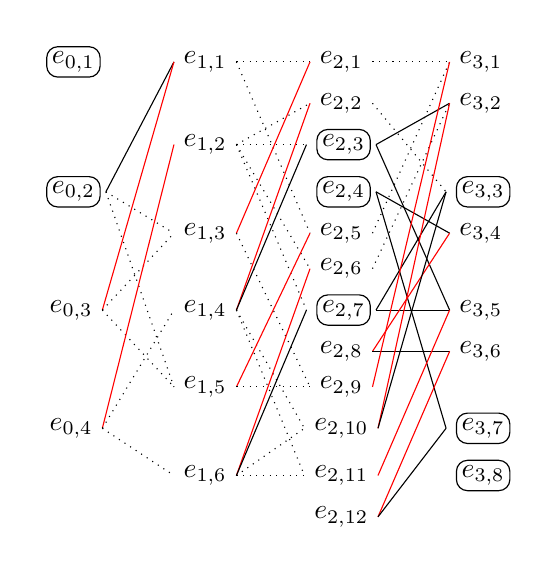
\begin{tikzpicture}\matrix (m) [matrix of math nodes, row sep=-1pt, column sep=25pt]{
\ccircled{$e_{0,1}$}&    e_{1,1}& e_{2,1}				& e_{3,1}\\
					&  			& e_{2,2}				& e_{3,2}\\
					& 	 e_{1,2}& \ccircled{$e_{2,3}$}	& \\
\ccircled{$e_{0,2}$}&  			& \ccircled{$e_{2,4}$}	& \ccircled{$e_{3,3}$}\\
					& 	 e_{1,3}& e_{2,5}				& e_{3,4}\\
					&  			& e_{2,6}				& \\
e_{0,3}				& 	 e_{1,4}& \ccircled{$e_{2,7}$}	& e_{3,5}\\
					&  			& e_{2,8}				& e_{3,6}\\
					&    e_{1,5}& e_{2,9}				& \\
e_{0,4}				&  			&e_{2,10}				& \ccircled{$e_{3,7}$}\\
					&    e_{1,6}&e_{2,11}				& \ccircled{$e_{3,8}$}\\
					&  			&e_{2,12}				&  \\};
\draw(m-4-1.east)--(m-1-2.west); 	  \draw[dotted](m-4-1.east)--(m-5-2.west); \draw[dotted](m-4-1.east)--(m-9-2.west); 
\draw[red](m-7-1.east)--(m-1-2.west); \draw[dotted](m-7-1.east)--(m-5-2.west); \draw[dotted](m-7-1.east)--(m-9-2.west); 
\draw[red](m-10-1.east)--(m-3-2.west);\draw[dotted](m-10-1.east)--(m-7-2.west);\draw[dotted](m-10-1.east)--(m-11-2.west); 
\draw[dotted](m-1-2.east)--(m-1-3.west); \draw[dotted](m-1-2.east)--(m-5-3.west); 
\draw[dotted](m-3-2.east)--(m-2-3.west); \draw[dotted](m-3-2.east)--(m-3-3.west); \draw[dotted](m-3-2.east)--(m-6-3.west); \draw[dotted](m-3-2.east)--(m-7-3.west); 
\draw[red](m-5-2.east)--(m-1-3.west); \draw[dotted](m-5-2.east)--(m-9-3.west); 
\draw[red](m-7-2.east)--(m-2-3.west); \draw(m-7-2.east)--(m-3-3.west); \draw[dotted](m-7-2.east)--(m-10-3.west); \draw[dotted](m-7-2.east)--(m-11-3.west); 
\draw[red](m-9-2.east)--(m-5-3.west); \draw[dotted](m-9-2.east)--(m-9-3.west); 
\draw[red](m-11-2.east)--(m-6-3.west); \draw(m-11-2.east)--(m-7-3.west); \draw[dotted](m-11-2.east)--(m-10-3.west); \draw[dotted](m-11-2.east)--(m-11-3.west); 
\draw[dotted](m-1-3.east)--(m-1-4.west); 
\draw[dotted](m-2-3.east)--(m-4-4.west); 
\draw(m-3-3.east)--(m-2-4.west); \draw(m-3-3.east)--(m-7-4.west); 
\draw(m-4-3.east)--(m-5-4.west); \draw(m-4-3.east)--(m-10-4.west);  
\draw[dotted](m-5-3.east)--(m-1-4.west); 
\draw[dotted](m-6-3.east)--(m-2-4.west); 
\draw(m-7-3.east)--(m-4-4.west); \draw(m-7-3.east)--(m-7-4.west); 
\draw[red](m-8-3.east)--(m-5-4.west); \draw(m-8-3.east)--(m-8-4.west); 
\draw[red](m-9-3.east)--(m-1-4.west); 
\draw[red](m-10-3.east)--(m-2-4.west); \draw(m-10-3.east)--(m-4-4.west); 
\draw[red](m-11-3.east)--(m-7-4.west); 
\draw[red](m-12-3.east)--(m-8-4.west); \draw(m-12-3.east)--(m-10-4.west); 
\end{tikzpicture}                       \hspace{12mm}
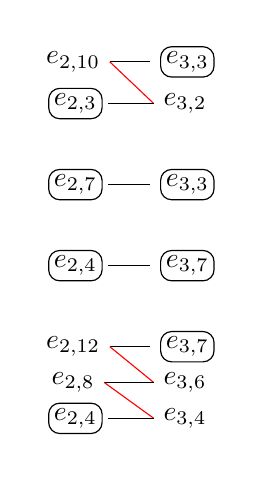
\begin{tikzpicture}\matrix (m) [matrix of math nodes, row sep=-3pt, column sep=15pt]{
e_{2,10}			&\ccircled{$e_{3,3}$}\\
\ccircled{$e_{2,3}$}&e_{3,2}\\[5mm]
\ccircled{$e_{2,7}$}&\ccircled{$e_{3,3}$}\\[5mm]
\ccircled{$e_{2,4}$}&\ccircled{$e_{3,7}$}\\[5mm]
e_{2,12}			&\ccircled{$e_{3,7}$}\\
e_{2,8}				&e_{3,6}\\
\ccircled{$e_{2,4}$}&e_{3,4}\\};
\draw(m-1-1.east)--(m-1-2.west); \draw[red](m-1-1.east)--(m-2-2.west); \draw(m-2-1.east)--(m-2-2.west);
\draw(m-3-1.east)--(m-3-2.west); \draw(m-4-1.east)--(m-4-2.west);
\draw(m-5-1.east)--(m-5-2.west); \draw[red](m-5-1.east)--(m-6-2.west); \draw(m-6-1.east)--(m-6-2.west); 
\draw[red](m-6-1.east)--(m-7-2.west); \draw(m-7-1.east)--(m-7-2.west);
\end{tikzpicture}
\begin{tikzpicture}\matrix (m) [matrix of math nodes, row sep=-3pt, column sep=15pt]{
	\partial_\gamma\!:\\[3mm]
	1\!\cdot\!\frac{-\!1}{1}\!\cdot\!1=-1\\[6mm]
	1\\[7mm]
	1\\[14.5mm]
	1\!\cdot\!\frac{-\!1}{1}\!\cdot\!1\!\cdot\!\frac{-\!1}{1}\!\cdot\!1=1\\
	};
\end{tikzpicture}\vspace{-2mm}\]
From this, we get an h-equivalent complex $C'_\ast\!: R^2\!
\xleftarrow{\,0\,}\!R^0\!
\xleftarrow{\,0\,}\!R^3\!
\xleftarrow{\!\!\left[\!\begin{smallmatrix}\mns1\!&0&0\\0&2&0\\1&0&0\end{smallmatrix}\!\right]\!\!}\!R^3\!$. 
Moreover, $f_\ast\!=\!\left[\!\begin{smallmatrix}1&0\\0&1\\0&0\\0&0\end{smallmatrix}\!\right]\!\!, 0,\! \left[\!\begin{smallmatrix}0&0&0\\\mns1&0&0\\1&0&0\\0&1&0\\0&0&0\\0&0&\mns1\\0&0&1\\0&0&0\\0&0&0\\0&0&0\\0&0&0\\0&0&0\end{smallmatrix}\!\right]\!\!,\! \left[\!\begin{smallmatrix}0&0&0\\\mns1&0&0\\1&0&0\\0&1&0\\0&0&0\\0&\mns1&0\\0&1&0\\0&0&1\\\end{smallmatrix}\!\right]$ and $g_\ast\!=\! 
\left[\!\begin{smallmatrix}1&0&0&0\\0&1&\mns1&0\end{smallmatrix}\!\right]\!\!, 0,\!
\left[\!\begin{smallmatrix}0&0&1&0&0&0&0&0&0&\mns1&\mns1&0\\ 
0&0&0&1&0&0&0&\mns1&0&0&0&1\\ 0&0&0&0&0&0&1&0&0&0&\mns1&0\end{smallmatrix}\!\right]\!\!, 
\left[\!\begin{smallmatrix}0&0&1&0&0&0&0&0\\0&0&0&0&0&0&1&0\\0&0&0&0&0&0&0&1\end{smallmatrix}\!\right]\!$. Thus over $R\!=\!\Z$, the homology and its generators are $H_0C_\ast\!=\! \langle e_{0,1},e_{0,2}\!-\!e_{0,3}\rangle \!\cong\!\Z^2\!$, $H_1C_\ast\!=\!0$, $H_2C_\ast\!=\! \langle e_{2,3}\!-\!e_{2,2},e_{2,4}\rangle \!\cong\!\Z\!\oplus\!\Z_2$, $H_3C_\ast\!=\!\langle e_{3,8}\rangle\!\cong\!\Z$. \hfill$\lozenge$\vspace{2mm}

\subsection{Remarks}\label{1.3.rmk} \textbf{(a)} If $C_\ast$ is the Poincar\'{e} chain complex of a finite simplicial complex $\Delta$ (or regular CW-complex), then $\Gamma_{\!C_\ast}$ is the Hasse diagram of $\Delta$ and AMT reduces to Forman's DMT \cite{citearticleFormanUGDMT} (discrete Morse theory, 1995). However, DMT gives a topological h-equivalence of CW-complexes $\Delta\!\simeq\!\Delta'$, not just an algebraic $C_\ast\!\simeq\!C'_\ast$. However, to determine the gluing maps, one needs to take into account paths between all critical simplices, not just those in consecutive degree; see \cite{citearticleNandaDMTCS}. \\[3pt]
\textbf{(b)} Notice that $\partial'_k$ is determined by $\partial_{k-_{\!}1},\partial_k,\partial_{k+1}$, not just $\partial_k$. Indeed, $I'_k$ is obtained from $\partial_{k-_{\!}1},\partial_k$ and $I'_{k+1}$ is obtained from $\partial_k,\partial_{k+1}$, whilst $\partial'_k$ is computed from $I'_k,I'_{k+1},\mathcal{M}_k,\partial_k$. Also, $\partial'_k$ and $f_k(v')\!=\!v'\!+\! \sum_{v\in I_k^+\!,\gamma\in\Gamma_{\!v'\!\!,v}}\!\partial_\gamma(v')$ contain only edges from $\partial_k$. On the other hand, $g_k(v)\!=\!v$ if $v\!\in\!I'_k$,\, and $g_k(v)\!=\!0$ if $v\!\in\!I^+_k$,\, and $g_k(v)\!=\!\sum_{v'\in I'_k,\gamma\in\Gamma_{\!v,v'}}\!\partial_\gamma(v)$ if $v\!\in\!I^-_k$, so $g_k$ contains only edges from $\partial_{k+1}$. \\[3pt]
\textbf{(c)} For every $u\!\leftarrow\!v\in\mathcal{M}_k$, no edge $x\!\leftarrow\!u$ or $v\!\leftarrow\!y$ can lie on a path between critical vertices in $\Gamma_{\!C_\ast}^{\mathcal M}$, since $\mathcal{M}$ is a matching. Thus we can delete all entries in the $u$-column (or $I_{k-\!1}^-$-columns) of $\partial_{k-\!1}$ and $v$-row (or $I_k^+$-rows) of $\partial_{k+1}$, without changing the computed complex $C'_\ast$ and h-equivalence $f_\ast,g_\ast$ (using the same $\mathcal{M}$). Also, for every $u\!\overset{w}{\leftarrow}\!v \in\mathcal{M}_k$ we can replace $u$ with $\frac{-\!1}{w}u$, i.e. multiply the $u$-row of $\partial_k$ by $\frac{-\!1}{w}$, and get an isomorphic complex, where edges of $\mathcal{M}$ in $\Gamma_{C_\ast}^{\mathcal{M}}$ have weight $1$. \\[3pt]
\textbf{(d)} As long as $\partial_\ast$ contains at least one invertible entry, by the construction below we always have a nonempty $\mathcal{M}_\leq$; see \ref{3.ordering}. Hence there is a sequence of h-equivalences\vspace{-1mm} 
\[C_\ast\!\overset{\;f'_\ast}{\longleftarrow}C'_\ast\!\overset{\;f''_\ast}{\longleftarrow}C''_\ast\!\longleftarrow\!\ldots\! \overset{\;\;f^{(r)}_\ast}{\longleftarrow}\!C^{(r)}_\ast\!\!, \tag{5} \label{(5)}\vspace{-1mm}\]
where all entries of $\partial_\ast^{(r)}$ are nonunits. If $R$ is a field, we have $\partial_\ast^{(r)}\!\!=\!0$, so $C^{(r)}_k\!\cong\!H_k C_\ast$; then $f_\ast\!:=\! f_\ast'\!\circ\!f_\ast''\!\circ\!\ldots\!\circ\!f_\ast^{(r)}$ gives the actual generators of homology in $C_\ast$; see \ref{5.1.algorithm}.\\[3pt]
\textbf{(e)} If $R_{(p)}$ is a localization of a PID $R$ at a prime $p$, then the only noninvertible entries are multiples of $p$. Hence $\partial_\ast^{(r)}\!=\!p^{a}\widetilde{\partial}_\ast^{(r)}$ for some $a\!\in\!\N$ and $\widetilde{\partial}_\ast^{(r)}$. Via \ref{AMT}\,(b) we can reconstruct $H_\ast(C^{(r)}_\ast\!\!,\partial^{(r)}_\ast)$ from $H_\ast(C^{(r)}_\ast\!\!,\frac{\partial^{(r)}_\ast}{p^a})$. Hence we continue with (\ref{(5)}) on \smash{$(C^{(r)}_\ast\!\!,\frac{\partial^{(r)}_\ast}{p^a})$}: for every Morse matching $\mathcal{M}$ on it, we add \smash{$(\frac{R}{Rp^{a}})^{|\mathcal{M}_k|}$} to $H_{k_{\!}-\!1}(C_\ast,\partial_\ast)$. This process ends at $\partial_\ast^{(r_{\!1}\!+\ldots+r_{\!t})}\!\!=\!0$, and we obtain the $p$-torsion of $H_{\!\ast}(C_{\!\ast};_{\!}R)$; see \ref{4.nonunits}. \vspace{4mm}

\section{Matchings induced from orderings}
In this section, we define a class of matchings on any chain complex. The construction requires (and is very dependent on) the ordering of basis elements. %\\[1mm]

\subsection{Formulation} Pick a total order $\leq_k$ on $I_k$ and let $\leq\,=\bigcup_k\!\leq_k$ be the combined partial order on the vertices of $\Gamma_{C_\ast}$. Visualize the elements of $I_k$ positioned vertically, with $u$ above $v$ iff $u\!<\!v$ (as with row indices in the matrix $\partial_{k+1}$). Define 
$$\mathcal{M}_\leq=\Big\{u\!\overset{w}{\leftarrow}\!v;\, \begin{smallmatrix}\forall x\leftarrow v:\: x<u,\\ \forall u\leftarrow y:\: v<y\end{smallmatrix}\Big\}\cap
\Big\{u\!\overset{w}{\leftarrow}\!v;\, w\!\in\!R^{\times}\Big\},$$ the set of all steepest edges which also have invertible weights. The critical vertices are $I'_\ast\!=\!\Big\{v;
\begin{smallmatrix}\text{if }v\overset{r}{\leftarrow} u\text{ is steepest into }v\text{,\;\;\;\; then }r\in R\setminus R^\times\!\text{ or }\exists v'\!\leftarrow u\text{ with }v'>v,\\
                   \text{if }w\overset{s}{\leftarrow} v\text{ is steepest out of }v\text{, then }s\in R\setminus R^\times\!\text{ or }\exists w\leftarrow v'\text{ with }v'\!<v\end{smallmatrix}\Big\}$.
Visually, $$\mathcal{M}_\leq\!=\!\Big\{ \raisebox{-12pt}{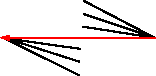
\includegraphics[width=0.17\textwidth]{steep-M.pdf}}\Big\}\text{ \;and\;
}I'_\ast\!=\! \Big\{v; \raisebox{-10pt}{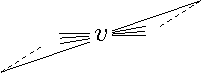
\includegraphics[width=0.22\textwidth]{steep-Mo.pdf}}\Big\}.$$

\begin{Lmm}\label{lmm1} \!\textbf{(a)}\! $\mathcal{M}_\leq$ is a Morse matching, the \emph{steepness} pairing associated to $\leq$.\\
\textbf{(b)} Every Morse matching is a subset of some steepness matching, so \vspace{-3pt}
$$\{\text{maximal Morse matchings on }\Gamma_{C_\ast}\} \subseteq \{\text{steepness pairings on }\Gamma_{C_\ast}\}.$$ %\vspace{-1mm}
\end{Lmm}\vspace{-1mm}
%We call such $\mathcal{M}$ the \emph{steepness} Morse matching associated to $C_\ast$, $I_k$, $\leq$.
\begin{proof} \textbf{(a)} The three conditions from the above definition must be verified.
\par $(1)$ $\mathcal{M}$ is a matching: For any edges
\!\!\raisebox{4pt}{$\xymatrixrowsep{-7pt}\xymatrixcolsep{14pt}
\xymatrix{&\scriptstyle x\ar[ld]\\\scriptstyle u&\\ &\scriptstyle y\ar[lu]\\}$}\!\!, either $x\!<\!y$ or $y\!<\!x$, so both edges cannot be in $\mathcal{M}$. For any edges \!\!\raisebox{4pt}{\smash{$\xymatrixrowsep{-7pt}\xymatrixcolsep{14pt} 
\xymatrix{\scriptstyle x&\\&\scriptstyle v\ar[ld]\ar[lu]\\ \scriptstyle y&\\}$}}\!\!, either $x\!<\!y$ or $y\!<\!x$, so both edges cannot be in $\mathcal{M}$. For any edges $x\!\overset{r}{\leftarrow}\!y\!\overset{s}{\leftarrow}\!z$, either $rs\!=\!0$ (then weights $r$ and $s$ are not units of $R$, so their edges cannot be in $\mathcal{M}$), or there exist edges $x\!\leftarrow\!v\!\leftarrow\!z$ with $y\!\neq\!v$ (otherwise $\partial_{k\!-\!1}\partial_k\!\neq\!0$). Now, either $y\!<\!v$ or $v\!<\!y$, so $x\!\leftarrow\!y$ and $y\!\leftarrow\!z$ cannot be both in $\mathcal{M}$, because at least one of them would not be the steepest.
\par $(2)$ $\mathcal{M}$ consists of isomorphisms: This is by the assumption on invertible weights.
\par $(3)$ $\mathcal{M}$ induces no cycles: Every zig-zag \!\!\raisebox{5pt}{$\xymatrixrowsep{-6pt}\xymatrixcolsep{12pt}
\xymatrix{&\scriptstyle x\ar[ld]\\ \scriptstyle u&\\ &\scriptstyle y\ar[lu]\\}$}\!\! in which $u\!\leftarrow\!x\in\mathcal{M}$ implies that $x\!<\!y$. Thus every zig-zag strictly increases the initial vertex, so a zig-zag path cannot end at its starting point, because it would imply $y\!>\!y$.\\
\textbf{(b)} Let $\mathcal{M}$ be an arbitrary Morse matching on $\Gamma_{C_\ast}$. It suffices to find for every $k$ a total order $\leq_k$ on $I_k$ such that the edges in $\mathcal{M}$ are the steepest.
\par By assumption, the digraph $\Gamma^{\mathcal{M}}_{C_\ast}$ is acyclic, so it can be viewed as a poset: $u\!\preceq\!v$ iff there exists a directed path from $u$ to $v$. Let $\preceq_k$ be the restriction of $\preceq$ to $I_k$. By construction, members of $\mathcal{M}$ are steepest w.r.t. $\preceq_k$. Since every finite partial order $\preceq_k$ can be extended to a linear order $\leq_k$, we conclude that $\mathcal{M}\!\subseteq\!\mathcal{M}_\leq$. 
\par If $\mathcal{M}$ is also maximal, then $\mathcal{M}\!\subseteq\!\mathcal{M}_\leq$ for some $\leq$ implies $\mathcal{M}\!=\!\mathcal{M}_\leq$.
\end{proof}
Note that if $\partial_k$ was infinite, with only diagonal and first supdiagonal entries which were all units, then $\mathcal{M}_\leq$ would not satisfy the part of condition $(3)$ about infinite paths. Thus infinite steepness pairings are not always Morse matchings.

\subsection{Matrix interpretation} If $\partial_k$ are given as finite matrices, we may assume that $I_k\!=\!\{1,\ldots,|I_k|\}$ and $\leq_k$ is the usual total order on $\N$, so the first row/column index is the smallest and the last one is the largest. Our $\mathcal{M}_\leq$ consists of those invertible matrix entries that have only zeros left in its row and below in its column, \vspace{-2mm}
\[\mathcal{M}_\leq=\left\{\raisebox{4.5pt}{$\scriptstyle u\,$}\!\!
\overset{\hspace{4pt}v}{\left[\hspace{-3pt}\begin{smallmatrix}~\\~\\~\\0\cdots0\rd{w}~~~\\ 
\hspace{15pt}0~~~\\[-1pt]
\hspace{14.5pt}\scalebox{0.8}{\rotatebox{90}{$.\hspace{0.4pt}.\hspace{0.4pt}.$}}~~~\\[-0.5pt]
\hspace{15pt}0~~~\\[2pt]\end{smallmatrix}\hspace{3pt}\right]}\!;\, w\!\in\!R^\times\!\!\right\}\!.
\tag{6} \label{(6)}\vspace{-1mm}\]
Thus $\mathcal{M}$ is largest when the matrices $\partial_k$ are in 'block upper-triangular' form. The set of critical vertices is $I_k'=I_k\!\setminus(\{\text{column indices of }\mathcal{M}_k\}\!\cup\!\{\text{row indices of }\mathcal{M}_{k+_{\!}1}\!\})$.
\begin{Lmm}\label{lmm2} Given $\mathcal{M}_\leq$, the $u'\!$-row  $r'$ of $\partial'_k$ is obtained from the $u'\!$-row $r$ of $\partial_k$ in the following way. While $V\!:=\!\{\text{nonzero positions of }r\}\!\cap\!I_k^+$ is nonempty, for $v\!=\!\min V$\!, $u\!\overset{w}{\leftarrow}\!v\in\mathcal{M}$, \smash{$u'\!\!\overset{\:w'}{\leftarrow}\!v\in\Gamma_{\!C_\ast}$}\!, add $\frac{-w'}{w}\!\cdot\!(u$-row of $\partial_k)$ to $r$. Then remove all $I_k^+$ entries (which are zero) and $I_{k+1}^-$-entries from $r$ to get the (shorter) row $r'$\!.
\end{Lmm}\vspace{-1mm}
Hence AMT gives the same result as Gaussian elimination with several pivots. However, with AMT we have to compute $\partial'(v)$ only for critical vertices $v$ (there may be very few of them, sometimes none at all). Also, AMT calculates the new complex recursively using (\ref{(4)}), which seems to be much faster than row operations.
\begin{proof} For the sake of clarity, we assume $\partial_k$ have block upper-triangular form, though the arguments work for any $\leq$. This is depicted by the image below: white area are zeros, full (vertical) lines are nonzeros, dashed (horizontal) lines and gray area are zeros and nonzeros, $\mathcal{M}_\leq$ consists of those red entries that are invertible, black bullets are nonzero entries, the dotted line is a path $\gamma$ from $v'$ to $u'$ in $\partial_k$.\vspace{-3mm}
\[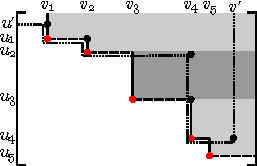
\includegraphics[width=0.5\textwidth]{steep-ord1.pdf} \tag{7} \label{(7)}\vspace{-2mm}\]
By the construction of $\Gamma_{\!C_\ast}^{\mathcal{M}}$, a path $\gamma\!\in\!\Gamma_{v'\!,u'\!}$ in $\partial_k$ consists of horizontal moves from black to red bullets, and vertical moves from red to black bullets. Let $I_k^+$ consist of $v_1,v_2,\ldots$. The $u'$-row of $\partial_k$ corresponds to paths in $\Gamma_{\!\ldots,u'}$ of length 1. Adding \smash{$\frac{-w_1'}{w_1}\!\cdot\!(u_1$}-row of $\partial_k)$ means replacing the path $u'\!\leftarrow\!v_1$ by all paths $u'\!\leftarrow\!v_1\!\to\!u_1\!\leftarrow\!v$ of length 3. Adding \smash{$\frac{-w_2'}{w_2}\!\cdot\!(u_2$}-row of $\partial_k)$ means replacing the latter by all paths $u'\!\leftarrow\!v_1\!\to\!u_1\!\leftarrow\!v_2\!\to\!u_2\!\leftarrow\!v$ of length 5. This process ends when all $v_1,v_2,\ldots$-entries of $r$ are zero (i.e. we used up all $\mathcal{M}_\leq$ to create paths), and then taking only the $I'_k$-entries (throwing away paths that do not begin in a critical $v'$) produces $r'$.
\end{proof}

\subsection{Examples}\label{2.3.exp} %In concrete cases, the steepness matching is effective (kills off most noncontributing vertices and there are few zig-zag paths), but a combinatorial description for $C'_\ast$ is usually hard to handle. 
\par $\bullet$ Consider the triangulation $\Delta$ below for the real projective plane. Let $C_\ast$ be the chain complex for simplicial homology of $\Delta$. The digraph $\Gamma_{C_\ast}$ (=Hasse diagram of $\Delta$) with the lexicographic order on vertices is pictured below left, and $\Gamma_{C_\ast}$ with a different total order is shown below that. The red edges are members of the steepness matching, the circled vertices are the critical simplices, and the dotted edges / gray entries can be deleted by remark \ref{1.3.rmk}\,(c).\vspace{-2mm}
\[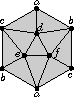
\includegraphics[width=0.23\textwidth]{steep-P2.pdf}\vspace{-7mm}\]
\[\hspace{-2mm}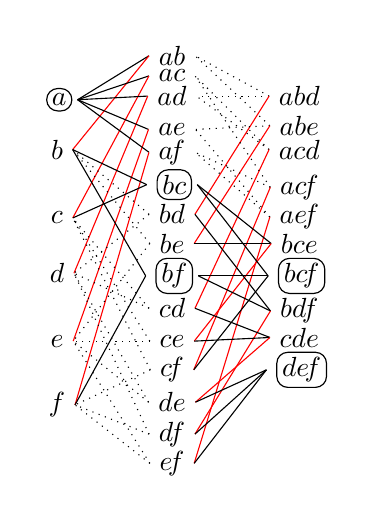
\begin{tikzpicture}\matrix (m) [matrix of math nodes, row sep=-5pt, column sep=25pt]{
 &ab&\\
 &ac&\\
\ccircled{$a$}&ad&abd\\
 &ae&abe\\
b&a\!f&acd\\
 &\ccircled{$bc$}&ac\!f\\
c&bd&ae\!f\\
 &be&bce\\
d&\ccircled{$b_{\!}f$}&\ccircled{$bc\!f$}\\
 &cd&bdf\\
e&ce&cde\\
 &c\!f&\ccircled{$de\!f$}\\
f&de&\\
 &df&\\
 &e\!f&\\ };
\draw(m-1-2.west)--(m-3-1.east);\draw[red](m-1-2.west)--(m-5-1.east); \draw(m-2-2.west)--(m-3-1.east);\draw[red](m-2-2.west)--(m-7-1.east);
\draw(m-3-2.west)--(m-3-1.east);\draw[red](m-3-2.west)--(m-9-1.east); \draw(m-4-2.west)--(m-3-1.east);\draw[red](m-4-2.west)--(m-11-1.east);
\draw(m-5-2.west)--(m-3-1.east);\draw[red](m-5-2.west)--(m-13-1.east);\draw(m-6-2.west)--(m-5-1.east);\draw(m-6-2.west)--(m-7-1.east);
\draw[dotted](m-7-2.west)--(m-5-1.east);  \draw[dotted](m-7-2.west)--(m-9-1.east); 
\draw[dotted](m-8-2.west)--(m-5-1.east);  \draw[dotted](m-8-2.west)--(m-11-1.east);
\draw(m-9-2.west)--(m-5-1.east);          \draw(m-9-2.west)--(m-13-1.east);
\draw[dotted](m-10-2.west)--(m-7-1.east); \draw[dotted](m-10-2.west)--(m-9-1.east);
\draw[dotted](m-11-2.west)--(m-7-1.east); \draw[dotted](m-11-2.west)--(m-11-1.east); 
\draw[dotted](m-12-2.west)--(m-7-1.east); \draw[dotted](m-12-2.west)--(m-13-1.east);
\draw[dotted](m-13-2.west)--(m-9-1.east); \draw[dotted](m-13-2.west)--(m-11-1.east); 
\draw[dotted](m-14-2.west)--(m-9-1.east); \draw[dotted](m-14-2.west)--(m-13-1.east);
\draw[dotted](m-15-2.west)--(m-11-1.east);\draw[dotted](m-15-2.west)--(m-13-1.east);
\draw[dotted](m-3-3.west)--(m-1-2.east);\draw[dotted](m-3-3.west)--(m-3-2.east);\draw[red](m-3-3.west)--(m-7-2.east);
\draw[dotted](m-4-3.west)--(m-1-2.east);\draw[dotted](m-4-3.west)--(m-4-2.east);\draw[red](m-4-3.west)--(m-8-2.east);
\draw[dotted](m-5-3.west)--(m-2-2.east);\draw[dotted](m-5-3.west)--(m-3-2.east);\draw[red](m-5-3.west)--(m-10-2.east);
\draw[dotted](m-6-3.west)--(m-2-2.east);\draw[dotted](m-6-3.west)--(m-5-2.east);\draw[red](m-6-3.west)--(m-12-2.east);
\draw[dotted](m-7-3.west)--(m-4-2.east);\draw[dotted](m-7-3.west)--(m-5-2.east);\draw[red](m-7-3.west)--(m-15-2.east);
\draw(m-8-3.west)--(m-6-2.east);\draw(m-8-3.west)--(m-8-2.east);\draw[red](m-8-3.west)--(m-11-2.east);
\draw(m-9-3.west)--(m-6-2.east);\draw(m-9-3.west)--(m-9-2.east);\draw(m-9-3.west)--(m-12-2.east);
\draw(m-10-3.west)--(m-7-2.east);\draw(m-10-3.west)--(m-9-2.east);\draw[red](m-10-3.west)--(m-14-2.east);
\draw(m-11-3.west)--(m-10-2.east);\draw(m-11-3.west)--(m-11-2.east);\draw[red](m-11-3.west)--(m-13-2.east);
\draw(m-12-3.west)--(m-13-2.east);\draw(m-12-3.west)--(m-14-2.east);\draw(m-12-3.west)--(m-15-2.east);
\end{tikzpicture}		\hspace{4mm} \raisebox{12mm}{$
R^6\!\xleftarrow{\!\!\!\left[\begin{smallmatrix}
	\mns1\!&\mns1\!&\mns1\!&\mns1\!&\mns1\!&0&\gr{0}&\gr{0}&0&\gr{0}&\gr{0}&\gr{0}&\gr{0}&\gr{0}&\gr{0}\\
	\rd{1}&0&0&0&0&\mns1\!&\gr{\mns1}\!&\gr{\mns1}\!&\mns1\!&\gr{0}&\gr{0}&\gr{0}&\gr{0}&\gr{0}&\gr{0}\\
	0&\rd{1}&0&0&0&1&\gr{0}&\gr{0}&0&\gr{\mns1}\!&\gr{\mns1}\!&\gr{\mns1}\!&\gr{0}&\gr{0}&\gr{0}\\
	0&0&\rd{1}&0&0&0&\gr{1}&\gr{0}&0&\gr{1}&\gr{0}&\gr{0}&\gr{\mns1}\!&\gr{\mns1}\!&\gr{0}\\
	0&0&0&\rd{1}&0&0&\gr{0}&\gr{1}&0&\gr{0}&\gr{1}&\gr{0}&\gr{1}&\gr{0}&\gr{\mns1}\!\\
	0&0&0&0&\rd{1}&0&\gr{0}&\gr{0}&1&\gr{0}&\gr{0}&\gr{1}&\gr{0}&\gr{1}&\gr{1}
	\end{smallmatrix}\right]\!\!\!}\! R^{15}\!\xleftarrow{\!\left[\begin{smallmatrix}
	\gr{1}&\gr{1}&\gr{0}&\gr{0}&\gr{0}&\gr{0}&\gr{0}&\gr{0}&\gr{0}&\gr{0}\\
	\gr{0}&\gr{0}&\gr{1}&\gr{1}&\gr{0}&\gr{0}&\gr{0}&\gr{0}&\gr{0}&\gr{0}\\
	\gr{\mns1}\!&\gr{0}&\gr{\mns1}\!&\gr{0}&\gr{0}&\gr{0}&\gr{0}&\gr{0}&\gr{0}&\gr{0}\\
	\gr{0}&\gr{\mns1}\!&\gr{0}&\gr{0}&\gr{1}&\gr{0}&\gr{0}&\gr{0}&\gr{0}&\gr{0}\\
	\gr{0}&\gr{0}&\gr{0}&\gr{\mns1}\!&\gr{\mns1}\!&\gr{0}&\gr{0}&\gr{0}&\gr{0}&\gr{0}\\
	0&0&0&0&0&1&1&0&0&0\\
	\rd{1}&0&0&0&0&0&0&1&0&0\\
	0&\rd{1}&0&0&0&\mns1\!&0&0&0&0\\
	0&0&0&0&0&0&\mns1\!&\mns1\!&0&0\\
	0&0&\rd{1}&0&0&0&0&0&1&0\\
	0&0&0&0&0&\rd{1}&0&0&\mns1\!&0\\
	0&0&0&\rd{1}&0&0&1&0&0&0\\
	0&0&0&0&0&0&0&0&\rd{1}&1\\
	0&0&0&0&0&0&0&\rd{1}&0&\mns1\!\\
	0&0&0&0&\rd{1}&0&0&0&0&1\\
\end{smallmatrix}\right]\!}\!R^{10}$}\vspace{-5mm}\]
\[\hspace{-2mm}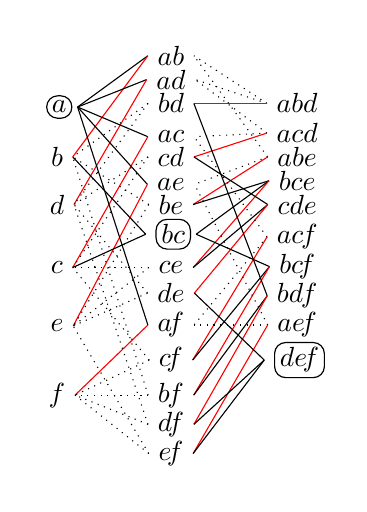
\begin{tikzpicture}\matrix (m) [matrix of math nodes, row sep=-5pt, column sep=25pt]{
 &ab&\\
 &ad&\\
\ccircled{$a$}&bd&abd\\
 &ac&acd\\
b&cd&abe\\
 &ae&bce\\
d&be&cde\\
 &\ccircled{$bc$}&ac_{\!}f\\
c&ce&bc\!f\\
 &de&bd_{\!}f\\
e&a\!f&ae\!f\\
 &c\!f&\ccircled{$de\!f$}\\
f&b_{\!}f&\\
 &df&\\
 &e\!f&\\};
\draw(m-1-2.west)--(m-3-1.east);\draw[red](m-1-2.west)--(m-5-1.east); 
\draw(m-2-2.west)--(m-3-1.east);\draw[red](m-2-2.west)--(m-7-1.east);
\draw[dotted](m-3-2.west)--(m-5-1.east);\draw[dotted](m-3-2.west)--(m-7-1.east); 
\draw(m-4-2.west)--(m-3-1.east);\draw[red](m-4-2.west)--(m-9-1.east);
\draw[dotted](m-5-2.west)--(m-7-1.east);\draw[dotted](m-5-2.west)--(m-9-1.east); 
\draw(m-6-2.west)--(m-3-1.east);\draw[red](m-6-2.west)--(m-11-1.east);
\draw[dotted](m-7-2.west)--(m-5-1.east);\draw[dotted](m-7-2.west)--(m-11-1.east); 
\draw(m-8-2.west)--(m-5-1.east);\draw(m-8-2.west)--(m-9-1.east);
\draw[dotted](m-9-2.west)--(m-9-1.east);\draw[dotted](m-9-2.west)--(m-11-1.east); 
\draw[dotted](m-10-2.west)--(m-7-1.east);\draw[dotted](m-10-2.west)--(m-11-1.east);
\draw(m-11-2.west)--(m-3-1.east);\draw[red](m-11-2.west)--(m-13-1.east); 
\draw[dotted](m-12-2.west)--(m-9-1.east);\draw[dotted](m-12-2.west)--(m-13-1.east);
\draw[dotted](m-13-2.west)--(m-5-1.east);\draw[dotted](m-13-2.west)--(m-13-1.east); 
\draw[dotted](m-14-2.west)--(m-7-1.east);\draw[dotted](m-14-2.west)--(m-13-1.east);
\draw[dotted](m-15-2.west)--(m-11-1.east);\draw[dotted](m-15-2.west)--(m-13-1.east);
\draw[dotted](m-3-3.west)--(m-1-2.east);\draw[dotted](m-3-3.west)--(m-2-2.east);\draw[red](m-3-3.west)--(m-3-2.east);
\draw[dotted](m-4-3.west)--(m-2-2.east);\draw[dotted](m-4-3.west)--(m-4-2.east);\draw[red](m-4-3.west)--(m-5-2.east);
\draw[dotted](m-5-3.west)--(m-1-2.east);\draw[dotted](m-5-3.west)--(m-6-2.east);\draw[red](m-5-3.west)--(m-7-2.east);
\draw(m-6-3.west)--(m-7-2.east);\draw(m-6-3.west)--(m-8-2.east);\draw[red](m-6-3.west)--(m-9-2.east);
\draw(m-7-3.west)--(m-5-2.east);\draw(m-7-3.west)--(m-9-2.east);\draw[red](m-7-3.west)--(m-10-2.east);
\draw[dotted](m-8-3.west)--(m-4-2.east);\draw[dotted](m-8-3.west)--(m-11-2.east);\draw[red](m-8-3.west)--(m-12-2.east);
\draw(m-9-3.west)--(m-8-2.east);\draw(m-9-3.west)--(m-12-2.east);\draw[red](m-9-3.west)--(m-13-2.east);
\draw(m-10-3.west)--(m-3-2.east);\draw(m-10-3.west)--(m-13-2.east);\draw[red](m-10-3.west)--(m-14-2.east);
\draw[dotted](m-11-3.west)--(m-6-2.east);\draw[dotted](m-11-3.west)--(m-11-2.east);\draw[red](m-11-3.west)--(m-15-2.east);
\draw(m-12-3.west)--(m-10-2.east);\draw(m-12-3.west)--(m-14-2.east);\draw(m-12-3.west)--(m-15-2.east);
\end{tikzpicture}		\hspace{4mm} \raisebox{12mm}{$
R^6\!\xleftarrow{\!\!\!\left[\begin{smallmatrix}
	\mns1\!& \mns1\!& \gr{0}& \mns1\!& \gr{0}& \mns1\!& \gr{0}& 0& \gr{0}& \gr{0}& \mns1\!& \gr{0}& \gr{0}& \gr{0}& \gr{0}\\
	\rd{1}& 0& \gr{\mns1}\!& 0& \gr{0}& 0& \gr{\mns1}\!& \mns1\!& \gr{0}& \gr{0}& 0& \gr{0}& \gr{\mns1}\!& \gr{0}& \gr{0}\\
	0& \rd{1}& \gr{1}& 0& \gr{1}& 0& \gr{0}& 0& \gr{0}& \gr{\mns1}\!& 0& \gr{0}& \gr{0}& \gr{\mns1}\!& \gr{0}\\
	0& 0& \gr{0}& \rd{1}& \gr{\mns1}\!& 0& \gr{0}& 1& \gr{\mns1}\!& \gr{0}& 0& \gr{\mns1}\!& \gr{0}& \gr{0}& \gr{0}\\
	0& 0& \gr{0}& 0& \gr{0}& \rd{1}& \gr{1}& 0& \gr{1}& \gr{1}& 0& \gr{0}& \gr{0}& \gr{0}& \gr{\mns1}\!\\
	0& 0& \gr{0}& 0& \gr{0}& 0& \gr{0}& 0& \gr{0}& \gr{0}& \rd{1}& \gr{1}& \gr{1}& \gr{1}& \gr{1}
	\end{smallmatrix}\right]\!\!\!}\! R^{15}\!\xleftarrow{\!\left[\begin{smallmatrix}
	\gr{1}& \gr{0}& \gr{1}& \gr{0}& \gr{0}& \gr{0}& \gr{0}& \gr{0}& \gr{0}& \gr{0}\\
	\gr{\mns1}\!& \gr{\mns1\!}& \gr{0}& \gr{0}& \gr{0}& \gr{0}& \gr{0}& \gr{0}& \gr{0}& \gr{0}\\
	\rd{1}& 0& 0& 0& 0& 0& 0& 1& 0& 0\\
	\gr{0}& \gr{1}& \gr{0}& \gr{0}& \gr{0}& \gr{1}& \gr{0}& \gr{0}& \gr{0}& \gr{0}\\
	0& \rd{1}& 0& 0& 1& 0& 0& 0& 0& 0\\
	\gr{0}& \gr{0}& \gr{\mns1}\!& \gr{0}& \gr{0}& \gr{0}& \gr{0}& \gr{0}& \gr{1}& \gr{0}\\
	0& 0& \rd{1}& \mns1\!& 0& 0& 0& 0& 0& 0\\
	0& 0& 0& 1& 0& 0& 1& 0& 0& 0\\
	0& 0& 0& \rd{1}& \mns1\!& 0& 0& 0& 0& 0\\
	0& 0& 0& 0& \rd{1}& 0& 0& 0& 0& 1\\
	\gr{0}& \gr{0}& \gr{0}& \gr{0}& \gr{0}& \gr{\mns1}\!& \gr{0}& \gr{0}& \gr{\mns1}\!& \gr{0}\\
	0& 0& 0& 0& 0& \rd{1}& 1& 0& 0& 0\\
	0& 0& 0& 0& 0& 0& \rd{\mns1}\!& \mns1\!& 0& 0\\
	0& 0& 0& 0& 0& 0& 0& \rd{1}& 0& \mns1\!\\
	0& 0& 0& 0& 0& 0& 0& 0& \rd{1}& 1
	\end{smallmatrix}\right]\!}\!R^{10}$}\vspace{-7mm}\]
By the first ordering, $C'_{\!\ast}\!=\! R\!\xleftarrow{\![\begin{smallmatrix}\!0&\!0\!\end{smallmatrix}]\!}\! R^2\!\xleftarrow{\!\!\left[\begin{smallmatrix}1&\mns1\\\!\mns1&\mns1\end{smallmatrix}\!\right]\!\!}\!R^2\!$, but by the second, $C'_{\!\ast}\!=\! R\!\xleftarrow{\![0]\!}\! R\!\xleftarrow{\![\mns2]\!}\!R$, with 3 critical simplices and 4 zig-zag paths, which is optimal. %Over $R\!=\!\Z$, this implies $H_\ast C_\ast\cong \Z,\,\Z_2,\,0$.
\par $\bullet$ In the example \ref{1.2.exp}, our $\mathcal{M}$ is the steepness matching.
\par $\bullet$ Sk\"{o}ldberg's matching in \cite[p.48]{citearticleSkoldbergMTFAV}, which computes the homology of Heisenberg Lie algebras, is $\mathcal{M}_\leq$ w.r.t. lexicographic ordering for $x_1\!\!<\!\ldots\!<\!x_n\!<\!y_1\!\!<\!\ldots\!<\!y_n$.
\par $\bullet$ Forman's matching in \cite[p.17]{citearticleFormanUGDMT}, which computes the homology of the simplicial complex on $E(K_n)$ of non-connected subgraphs of the full graph $K_n$, is $\mathcal{M}_\leq$ w.r.t. the lexicographic order using $12\!<\!13\!<\!23\!<\!14\!<\!24\!<\!34\!<\!15\!<\!\ldots\!<\!45\!<\!\ldots$.
\par $\bullet$ Kozlov's matching in \cite[p.193]{citearticleKozlovCAT}, which computes the homology of the simplicial complex on $V(P_n)$ of all independent sets in the path graph $P_n$, is $\mathcal{M}_\leq$ w.r.t. the lexicographic order for $0\!<\!3\!<\!6\!<\!9\!<\!\ldots\!<\!2\!<\!5\!<\!8\!<\!11\!<\!\ldots\!<\!1\!<\!4\!<\!7\!<\!10\!<\!\ldots$. \hfill$\lozenge$

\subsection{Remarks}\label{2.4.rmk} Consider the following chain complexes of $\Z$-modules:\vspace{-4pt}
$$%(0)\; 0\!\leftarrow\!R^2\!\! \overset{\big[\!\begin{smallmatrix}1&1\\-\!1&1\end{smallmatrix}\!\big]}{\longleftarrow} \!\!R^2\!\leftarrow\!0\;\;\;
(a)\; 0\!\leftarrow\!\Z^2\!\! \overset{\big[\!\begin{smallmatrix}3&4\\2&3\end{smallmatrix}\!\big]}{\longleftarrow} \!\!\Z^2 \!\leftarrow\!0\hspace{9mm}
(b)\; 0\!\leftarrow\!\Z^n\!\! \xleftarrow{\!\!\left[\!\!\begin{smallmatrix}
&&\hspace{-3pt}1&\hspace{-2pt}1\\%[-5pt]
&\hspace{-6pt}\rotatebox[origin=c]{100}{$\ddots$}\hspace{-4pt} &\hspace{-12pt}\rotatebox[origin=c]{100}{$\ddots$}\hspace{-4pt}&\\[-2pt]
&\hspace{-8pt}1&\hspace{-12pt}1&\\
\,1&\hspace{-7pt}1&&\\[0pt]
\,\rd{1}&&&\\[2pt]\end{smallmatrix}\!\right]\!\!} \!\!\Z^n \!\!\leftarrow\!0\hspace{9mm}
(c)\; 0\!\leftarrow\!\Z^2 \!\!\overset{\big[\!\begin{smallmatrix}0&\!1\\\rd{1}&\!1\end{smallmatrix}\!\big]}{\longleftarrow}\!\!\Z^2 \!\leftarrow\!0\vspace{-5pt}$$
%\par$\bullet$ In general, there exist chain complexes of free modules, which are contractible, but do not admit a Morse matching (w.r.t. the standard basis) with no critical vertices. For example, $(0)$ is contractible when $2$ is a unit of $R$ (since $0\!\leftarrow\!M\!\overset{f}{\leftarrow}\!N\!\leftarrow\!0$ is contractible iff $f$ is an isomorphism, with the homotopy being $f^{-1}$). But its digraph $\Gamma_{C_\ast}$ is $\begin{tikzpicture}\matrix (m) [matrix of math nodes, row sep=3pt, column sep=10pt]{
%\scriptscriptstyle x&\scriptscriptstyle a\\
%\scriptscriptstyle y&\scriptscriptstyle b\\};
%\draw(m-1-1.east)--(m-1-2.west);\draw(m-1-1.east)--(m-2-2.west);\draw(m-2-1.east)--(m-1-2.west);\draw(m-2-1.east)--(m-2-2.west);
%\end{tikzpicture}$, which shows that if a matching $\mathcal{M}$ contains two edges, it necessarily induces cycles in $\Gamma^\mathcal{M}_{C_\ast}$. However, choosing a different basis gives the digraph $\begin{tikzpicture}\matrix (m) [matrix of math nodes, row sep=3pt, column sep=10pt]{
%\scriptscriptstyle x+y&\scriptscriptstyle a\\
%\scriptscriptstyle   y&\scriptscriptstyle b\\};
%\draw(m-1-1.east)--(m-1-2.west);\draw(m-2-1.east)--(m-1-2.west);\draw(m-2-1.east)--(m-2-2.west);
%\end{tikzpicture}$ on which the Morse matching $\mathcal{M}\!=\!\{x\!+\!y\!\to\!a,y\!\to\!b\}$ kills everything. This suggests that one should be careful when picking bases of modules in the chain complex to construct a matching.
\par$\bullet$ The boundary matrices might have all entries non-invertible (so the steepness matching is empty w.r.t. any ordering), yet the chain complex can still be contractible. E.g. $(a)$ is contractible (since $\det\partial_1\!=\!1\!\in\!\Z^\times$), but  $\mathcal{M}_\leq\!=\!\emptyset$.
\par$\bullet$ The boundary matrices may have all nonzero entries invertible and be very sparse, but if $\leq$ is badly chosen, the steepness matching can still be very small. E.g. for $(b)$ our $\mathcal{M}\!=\!\{n\!\leftarrow\!1\}$ has one edge. However, if we pick the same order on rows and reverse order on columns, $\partial_1$ becomes upper-triangular and $\mathcal{M}\!=\!\{i\!\leftarrow\!i;\,i\!\in\![n]\}$.
\par$\bullet$ The inclusion in Lemma \ref{lmm1}\,(b) is not an equality. E.g. for $(c)$ the steepness pairing $\mathcal{M}\!=\!\{2\!\leftarrow\!1\}$ is not maximal. It is strictly contained in the Morse Matching $\mathcal{M}\!=\!\{2\!\leftarrow\!1,1\!\leftarrow\!2\}$, which is the steepness pairing when the rows are switched.
\par$\bullet$ The boundary matrices may have all nonzero entries invertible, but the steepness matching could be small no matter the choice of the ordering. E.g. for the complex \smash{$0\!\leftarrow\!\Z^m\!\! \overset{\partial}{\longleftarrow} \!\!\Z^n \!\leftarrow\!0$} in which every entry of $\partial$ is $\pm1$, any choice of $\leq$ gives $\mathcal{M}\!=\!\{m\!\leftarrow\!1\}$, though admittedly this matrix $\partial$ is not sparse.
\par$\bullet$ Needless to say, for most chain complexes in practice, e.g. those coming from simplicial complexes (Poincar\'{e}), (semi)groups (Eilenberg-MacLane), associative algebras (Hochschild), Lie algebras (Chevalley), knots and links (Khovanov), etc., the matrices are usually very sparse, with just entries $0$ and $\pm1$. Hence the steepness matching is very large and useful, as it kills the majority of basis elements. \hfill$\lozenge$\vspace{4mm}

\section{Choice of ordering}\label{3.ordering}
When $\partial_k$ are given as finite matrices, the bases and orders are already determined: $I_k\!=\!\{1,\ldots,|I_k|\}$ and $\leq_k$=(usual total order on $\N)$. We can get any other order by permuting the rows and/or columns of boundary matrices. 
\par Even in very sparse complexes, bad orders lead to small matchings and therefore slow computation (as seen in remark \ref{2.4.rmk}\,$(b)$), or they lead to increase in matrix densities and therefore memory overflow (as seen in the following example).
\subsection{Examples}\label{3.1.exp} Consider the 3 orderings of the same chain complex:\vspace{-3pt}
\[\hspace{-5pt}C_{\!\ast}\!:\; \; \overset{\raisebox{5mm}{$\displaystyle(a)$}}{0}\!\!\leftarrow\!\Z^m\!\! \xleftarrow{\!\!\left[\!\begin{smallmatrix} 1&\\[-0pt]\scalebox{0.8}{\rotatebox{90}{$.\hspace{0.4pt}.\hspace{0.4pt}.$}}&&\!0\!\\1\\\rd{1}&\!1\!&\!\cdots\!&\!1 \end{smallmatrix}\!\right]\!\!} \!\!\Z^n \!\!\leftarrow\!0\hspace{7mm}
\overset{\raisebox{5mm}{$\displaystyle(b)$}}{0}\!\!\leftarrow\!\Z^m\!\! \xleftarrow{\!\!\left[\!\begin{smallmatrix} \!1\!&\!1\!&\!\cdots\!&\!1\\1\\\scalebox{0.8}{\rotatebox{90}{$.\hspace{0.4pt}.\hspace{0.4pt}.$}}&&\!0\!\\\rd{1}&\\ \end{smallmatrix}\!\right]\!\!} \!\!\Z^n \!\!\leftarrow\!0\hspace{7mm}
\overset{\raisebox{5mm}{$\displaystyle(c)$}}{0}\!\!\leftarrow\!\Z^m\!\! \xleftarrow{\!\!\left[\!\begin{smallmatrix} \rd{1}\!&\!\cdots\!&\!1\!&\!1\\&&&\!1\\&\!0\!&&\!\scalebox{0.8}{\rotatebox{90}{$.\hspace{0.4pt}.\hspace{0.4pt}.$}}\\&&&\!\rd{1}\\\end{smallmatrix}\!\right]\!\!} \!\!\Z^n \!\!\leftarrow\!0\vspace{-2mm}\]
\[\hspace{-5pt}C'_{\!\ast}\!:\; 0\!\leftarrow\!\Z^{m_{\!}-_{\!}1}\!\! \xleftarrow{\!\!\left[\!\begin{smallmatrix} \mns1&\!\cdots\!&\mns1\\[-0pt]\scalebox{0.8}{\rotatebox{90}{$.\hspace{0.4pt}.\hspace{0.4pt}.$}}& &\scalebox{0.8}{\rotatebox{90}{$.\hspace{0.4pt}.\hspace{0.4pt}.$}}\\
	\mns1&\!\cdots\!&\mns1\end{smallmatrix}\!\right]\!\!} \!\!\Z^{n_{\!}-_{\!}1} \!\!\!\leftarrow\!0\hspace{5mm}
0\!\leftarrow\!\Z^{m_{\!}-_{\!}1}\!\! \xleftarrow{\!\!\left[\!\begin{smallmatrix} 1\!&\!\cdots\!&\!1\\&\phantom{0}\\&\!0\!\\\end{smallmatrix}\!\right]\!\!} \!\!\Z^{n_{\!}-_{\!}1} \!\!\!\leftarrow\!0\hspace{5mm}
0\!\leftarrow\!\Z^{m_{\!}-_{\!}2}\!\! \xleftarrow{\!\!\left[\!\begin{smallmatrix} &\!\phantom{a}\!&\\\!\phantom{a}\!&\!0\!&\!\phantom{a}\!\\&\!\phantom{a}\!& \\\end{smallmatrix}\!\right]\!\!} \!\!\Z^{n_{\!}-_{\!}2} \!\!\!\leftarrow\!0\vspace{-0mm}\]
If in $(a)$ we switch the first and last row, we get $(b)$; if we also switch the first and last column, we get $(c)$. The starting matrix density is $\frac{m+n-1}{mn}$. After computing $C'_\ast$, in $(a)$ the density increased to $1$, in $(b)$ it decreased to $\frac{1}{m\!-\!1}$, and in $(c)$ it became $0$. \hfill$\lozenge$\\

\subsection{Algorithm} To meaningfully reduce $C_\ast$, we must create as many red entries like in (\ref{(6)}), as few situations like in example \ref{3.1.exp}\,$(a)$, and as few zig-zag paths like in (\ref{(7)}) (i.e. new entries in $C'_\ast$) as possible. This is achieved in two steps: 
\[\begin{tabular}{l}For $k\!=\!1,\ldots,N$, permute the columns of $\partial_k$ (and thus rows of $\partial_{k+1}$, with \\ 
the same permutation), by lexicographically comparing, for every column\\
index $v$, the tuple $\big(c_1,c_2,c_3,c_4\big)(v)$. Here we used:\\ 
$c_1$ = 0 if the $v$-column contains a unit entry and 1 otherwise,\\
$c_2$ = position of the last nonzero entry in the $v$-column,\\
$c_3$ = density of the $v$-column,\\
$c_4$ = 0 if the last nonzero entry in the $v$-column is a unit and 1 otherwise.\end{tabular} \tag{8} \label{(8)}\vspace{-0mm}\] 
\[\begin{tabular}{l}For $k\!=\!N\!-\!a,N\!-\!a\!-\!b,N\!-\!a\!-\!2b,N\!-\!a\!-\!3b,\ldots$ where $a\!\in\!\{0,1\}$, permute\hspace{0pt}\phantom{.}\\
the rows of $\partial_k$ (and thus columns of $\partial_{k-1}$, with the same permutation),\\ 
by lexicographically comparing, for every row index $u$, \\
the tuple $\big(r_1,r_2,r_3,r_4\big)(u)$. Here we used:\\ 
$r_1$ = 1 if the $u$-row contains a unit entry and 0 otherwise,\\
$r_2$ = position of the first nonzero entry in the $u$-row,\\
$r_3$ = -(density of the $u$-row),\\
$r_4$ = 1 if the first nonzero entry in the $u$-row is a unit and 0 otherwise.\end{tabular} \tag{9} \label{(9)}\vspace{-0mm}\] 
Performing (\ref{(9)}) for $a\!=\!0$ and $b\!=\!1$ by comparing just $r_2$ produces a complex, in which every matrix has the form (\ref{(7)}). Similarly, applying (\ref{(8)}) by comparing just $c_2$ produces a complex, in which every matrix has the form (\ref{(10)}) below (white area are zeros, gray area and dashed lines are any entries, full lines are nonzeros, invertible red entries are members of $\mathcal{M}_\leq$). Further comparing $r_i,\ldots$ (resp. $c_j,\ldots$) means permuting the rows (columns) in the dark gray area of (\ref{(7)}) (resp. (\ref{(10)})). 
\par As an illustration, notice that in examples \ref{2.3.exp}, the second ordering of the chain complex for the projective plane has the form (\ref{(7)}).\vspace{-1mm}
\[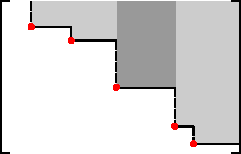
\includegraphics[width=0.5\textwidth]{steep-ord2.pdf} \tag{10} \label{(10)}\vspace{-2mm}\] 
\par If we apply (\ref{(8)}) and then (\ref{(9)}) for $a\!=\!0$ and $b\!=\!1$, then (\ref{(9)}) will not be reordering matrices of the form (\ref{(10)}), since it changes $\partial_k$ as well as $\partial_{k-1}$. However, if we apply (\ref{(8)}) and then (\ref{(9)}) for $a\!=\!\{0,1\}$ and $b\!=\!2$, then (\ref{(9)}) receives as input the form (\ref{(10)}).
\par If we want to maximize the size of $\mathcal{M}_\leq$, we order w.r.t. $(c_1,c_2,c_4)$ and $(r_1,r_2,r_4)$. If we want to minimize the density of matrices in $C'_\ast$, we order w.r.t. $(c_1,c_2,c_3)$ and $(r_1,r_2,r_3)$. Note however, that this does not always produce the desired result, since (\ref{(9)}) orders only half of the matrices, and may mess up the other half.

%\begin{Lmm}\label{lmm3} 
%\end{Lmm}\vspace{-1mm}
%\begin{proof}
%\end{proof}	

\subsection{Remark} In my experience, if the matrices of $C_\ast$ come from a typical homology theory (e.g. from simplicial complexes, groups, associative or Lie algebras, etc.), then the default lexicographic order is often already very effective. Without spending time on reordering, AMT produces a larger chain complex, but faster. %Thus applying AMT with reordering once and applying AMT without reordering several times produces a similar result.
\par It would be interesting if one could derive some nice characterization that tells for which $\leq$ is our stepness Morse matching $\mathcal{M}_\leq$ maximal.\vspace{4mm}

\section{Noninvertible entries}\label{4.nonunits}
Let $R$ be a PID and $p\!\in\!R$ a prime. Hence for every $k$, we have $H_k(C_\ast;R)\cong\bigoplus_{t\in T_k}R/(t)$ for a unique finite multiset $T_k$ of zeros and prime powers. Then over the localized ring, $H_k(C_\ast;R_{(p)}\!)\cong\bigoplus_{t\in T_k\cap Rp}R_{(p)}/(t)$ gives $p$-torsion and free part. Computing $H_k(C_\ast;R_{(p)}\!)$ for all (relevant) primes $p$ then produces $H_k(C_\ast;R)$.
\par The only noninvertible elements in the subring $R_{(p)}\!=\!\{\frac{a}{b}\!\in\!Q(R); b\!\notin\!Rp\}$ of the field of fractions of $R$ are $R^\times_{(p)}\!=\!\{\frac{a}{b}\!\in\!Q(R); a\!\in\!Rp,b\!\notin\!Rp\}$, the multiples of $p$.\\

\subsection{Algorithm}\label{4.1.algorithm} As long as a chain complex contains a unit entry $u\!\overset{w}{\leftarrow}\!v$, there is a Morse matching $\mathcal{M}$ containing that entry (e.g. $\mathcal{M}\!=\!\{u\!\overset{w}{\leftarrow}\!v\}$ suffices). 
\par Let $C_\ast^{[0]}\!:=\!C_\ast$. We have a sequence (\ref{(5)}), where $C_\ast^{(r)}$ contains only nonunit entries (i.e. multiples of $p$). Let $p^{a_1}$ be the largest power of $p$ that divides all nonzero entries of $C_\ast^{(r)}$ (if there are any). Let $C_\ast^{[1]}$ be the complex $C_\ast^{(r)}$ in which all entries are divided by $p^{a_1}$; then $C_\ast^{[1]}$ contains unit entries. Thus we can apply (\ref{(5)}) again, get a complex with all entries nonunits, divide it by the largest divisor $p^{a_2}$, and obtain a complex $C_\ast^{[2]}$ that contains unit entries. Doing the same again produces $C_\ast^{[3]}$ and so on. Denote by $m_{k,i}\!\in\!\N$ the sum of $|\mathcal{M}_k|$, where $\mathcal{M}$ are all the Morse matchings, used when applying (\ref{(5)}) to $C_\ast^{[i-1]}$ to create $C_\ast^{[i]}$.\vspace{-1mm}

\begin{Lmm}\label{lmm4} The above sequence of complexes terminates at some $C_\ast^{[t]}$ in which all matrices are zero. Then the $p$-torsion of $H_k(C_\ast;R)$ is $\bigoplus_{1\leq i<t}(R/\!Rp^{a_1+\ldots+a_i}\!)^{m_{k_{\!}+_{\!}1,i}}$\!.
\end{Lmm}\vspace{-1mm}
\begin{proof} The sequence terminates, since every $e\!\in\!\mathcal{M}_k$ reduces the finite rank of $C_k$ and $C_{k_{\!}-\!1}$ by 1. Via using \ref{AMT}\,(b) repetitively, the above procedure reconstructs the SNF of $C_\ast$ over $R_{(p)}$. Indeed, by constructing $C_\ast^{[1]}\!,\ldots,C_\ast^{[t]}$, we successively change the bases of all $C_k$, such that the boundary matrices have the form\vspace{-2mm}
\[\begin{array}{l}
\partial_k\!=\! \mathrm{diag}(\id_{m_{k,0}},0,p^{a_1}\partial_k^{[1]}),\\
\partial_k\!=\! \mathrm{diag}(\id_{m_{k,0}},0,p^{a_1}\id_{m_{k,1}},0,p^{a_{1\!}+a_2}\partial_k^{[2]}),\\
\partial_k\!=\! \mathrm{diag}(\id_{m_{k,0}},0,p^{a_1}\id_{m_{k,1}},0,p^{a_{1\!}+a_2}\id_{m_{k,2}},0,p^{a_{1\!}+a_2+a_3}\partial_k^{[3]}),\\[-5pt]
\hspace{14pt}\vdots\\[-3pt]
\partial_k\!=\! \mathrm{diag}(\id_{m_{k,0}},0,p^{a_1}\id_{m_{k,1}},0,\ldots,p^{a_{1\!}+\ldots+a_{t\!-\!1}}\id_{m_{k,t\!-\!1}},0,p^{a_{1\!}+\ldots+a_t}0),\vspace{-2mm}
\end{array}\]
where the last zero is the trivial map $C_{k_{\!}-\!1}^{[t]}\!\leftarrow\!C_k^{[t]}$ that determines the free part.\end{proof}

\subsection{Remark} In my experience, if the matrices of $C_\ast$ over $\Z$ have only entries $0$ and $\pm1$ and if the torsion part of $H_\ast C_\ast$ is small (relative to the ranks of $C_k$), then applying AMT produces $C'_\ast$ in which most entries are still $0$ and $\pm1$. Consequently, for many complexes  it is effective to work over $\Z$ directly, not over $\Z_{(p)}$ for all $p$.
\par For complexes $C_\ast$ with large torsion part in homology, it would really help if one could efficiently compute some finite (reasonably small) set of primes $P$, such that $H_\ast C_\ast$ contains no $p$-torsion for $p\!\in\!\N\!\setminus\!P$.\vspace{4mm}

\section{Computer Implementation} 

%\subsection{Parallelization}

\subsection{Algorithm}\label{5.1.algorithm} We have a procedure to compute everything from \ref{AMT}.\\[-3mm]
\begin{enumerate} \setlength{\itemindent}{-5mm} 
	\item[] Input: Matrices $\partial_\ast\!=\!(\partial_k)_{k=1}^N$ of the complex $C_\ast$ over $R$. Let $f_\ast\!:=\!(\id_k)_{k=0}^N$.
	\item[] While at least one matrix $\partial_k$ contains at least one invertible entry: 
	\begin{enumerate} \setlength{\itemindent}{-0mm} 
		\item[(a)] Permute the basis elements (columns/rows of all $\partial_k$), so that as many invertible entries have zeros left and below them, e.g. like (\ref{(8)}) and (\ref{(9)}).
		\item[(b)] Compute $\mathcal{M}_\leq$ using (\ref{(6)}). For all $k$, delete the $I_{k-\!1}^-$-columns of $\partial_{k-\!1}$ and $I_k^+$-rows of $\partial_{k+1}$, which are  unnecessary by remark \ref{1.3.rmk}\,(c).
		\item[(c)] Compute $\partial'_\ast$ and $f'_\ast$ w.r.t. $\mathcal{M}_\leq$ using formulas (\ref{(4)}) and \ref{1.3.rmk}\,(b) recursively (finding directed paths in a graph). 
		\item[(d)] Let $\partial_\ast\!:=\!\partial'_\ast$ and $f_k\!:=\!f_kf_k'$ (matrix multiplication).
	\end{enumerate}
	\item[] Return: $\partial'_\ast$ (the reduced chain complex) and $f_\ast$ (the h-equivalence $C'_\ast\!\to\!C_\ast$). 
\end{enumerate}
Step (a) is optional: if we use it, then this algorithm returns $\partial'_\ast$ in which all entries are nonunits. Also, there are many ways to perform (a), so it leaves a lot of room for optimization. If $R$ is a field, the above process returns $\partial'_\ast\!=\!0$; then the width of $\partial'_k$ equals $\dim H_kC_\ast$ and the columns of $f_k$ are the generators of $H_kC_\ast$, by (\ref{(5)}). 
\par When $\partial_k$ are sparse and come from common homology theories, the default $\leq$ is often quite good for computation, and additional reordering improves the calculation a little, but spends unnecessary time. Thus we often skip (a), unless we work over a local PID, which requires killing all unit entries to get torsion.
\par The part of (b) about column/row deletion is optional: if we skip it, the calculation will just require more time and memory. The part of (c) and (d) about $f_\ast$ is optional: if we only want the isomorphism type of $H_kC_\ast$, we compute just $\partial'_\ast$.

\subsection{Explicit code}\label{code}
Below is a rudimentary code in \textsc{Mathematica} that, given $C_\ast$ over $\Z$ or $\Q$ or $\Z_p$ for prime $p$, changes $C_\ast$ with the command \texttt{reduceChCx} (using the steepness matching) to a smaller h-equivalent complex according to AMT \ref{AMT}. It is to be copied into \textsc{Mathematica} and inspected there, hence the small font here.\\
%tft[status_]:=TableForm[Transpose@status,TableSpacing->\{0,0.5\},TableDepth->2];
%now:=With[\{d=DateList[]\![\![1;\!;-2]\!]\}\!,Framed[StringJoin[ToString/@\{d[\![1]\!]\!,"."\!,d[\![2]\!]\!,"."\!,d[\![3]\!]\!," "\!,d[\![4]\!]\!,":"\!,d[\![5]\!]\}]\!, 
%FrameMargins->1,ContentPadding->False,Background->GrayLevel[0.9]\!,BaseStyle->\{FontFamily->"Alegreya SC"\}]];
\begin{alltt}\tiny
\$HistoryLength=0; SetAttributes[\{steepM,orderC,orderR,reduceChCx\}\!,HoldAll];
cols[a_] := With[\{l=GatherBy[Sort@Transpose@Join[Reverse@Transpose@a["NonzeroPositions"]\!,\{a["NonzeroValues"]\}],
   First]\}\!, AssociationThread[Map[First\!,l\!,2],Map[Rest\!,l\!,\{2\}]]]; 
orderC[bdrs_,dims_] := Module[\{dim=Length@bdrs,cls,kys,v,c1,c2,c3,c4,pmt,pc,pr\}, Do[
   If[dims[\![k]\!]*dims[\![k+1]\!]==0 || bdrs[\![k]\!]["Density"]==0, Continue[]]; cls=cols@bdrs[\![k]\!]; v=Values@cls; 
   c1=If[MemberQ[Last/@#^2,1],0,1]&/@v; c2=Length/@v; c3=#[\![-1,1]\!]&/@v; c4=If[#[\![-1,2]\!]^2==1,0,1]&/@v; 
   kys=Keys@cls; Clear[cls,v]; pmt=First/@SortBy[Transpose@\{kys\!,c1\!,c3\!,c4\}\!,Rest]; pmt=AssociationThread[pmt\!,kys];
   pc=(\{u_,v_\}->w_):>(\{u,pmt[v]\}->w);   pr=(\{u_,v_\}->w_):>(\{Lookup[pmt,u,u],v\}->w);
   bdrs[\![k]\!]  =SparseArray[ArrayRules[bdrs[\![k  ]\!]][\![1;\!;-2]\!] /.pc,dims[\![k;\!;k+1]\!]];   If[k<dim,
   bdrs[\![k+1]\!]=SparseArray[ArrayRules[bdrs[\![k+1]\!]][\![1;\!;-2]\!] /.pr,dims[\![k+1;\!;k+2]\!]];], \{k,dim\}]]; 
orderR[bdrs_,dims_,a_,b_] := Module[\{dim=Length@bdrs,rws,kys,v,r1,r2,r3,r4,pmt,pr,pc\}, Do[
   If[dims[\![k]\!]*dims[\![k+1]\!]==0 || bdrs[\![k]\!]["Density"]==0, Continue[]]; rws=cols@Transpose@bdrs[\![k]\!]; v=Values@rws; 
   r1=If[MemberQ[Last/@#^2,1],1,0]&/@v; r2=-Length/@v; r3=#[\![1,1]\!]&/@v; r4=If[#[\![1,2]\!]^2==1,1,0]&/@v; 
   kys=Keys@rws; Clear[rws,v]; pmt=First/@SortBy[Transpose@\{kys,r1,r3,r4\},Rest]; pmt=AssociationThread[pmt,kys];
   pr=(\{u_,v_\}->w_):>(\{pmt[u],v\}->w); pc=(\{u_,v_\}->w_):>(\{u,Lookup[pmt,v,v]\}->w); 
   bdrs[\![k]\!]  = SparseArray[ArrayRules[bdrs[\![k  ]\!]][\![1;\!;-2]\!] /.pr, dims[\![k;\!;k+1]\!]]; If[1<k,
   bdrs[\![k-1]\!]= SparseArray[ArrayRules[bdrs[\![k-1]\!]][\![1;\!;-2]\!] /.pc, dims[\![k-1;\!;k]\!]];], \{k,dim-a,1,-b\}]];
steepM[rws_,cls_,p_:"Z"] := Module[\{v,w\}, Association@DeleteCases[Table[\{v,w\}=rws[u][\![1]\!]; If[cls[v][\![-1]\!]==\{u,w\}
   \&\& Which[p=="Z",w^2==1,p==0,w!=0,True,Mod[w,p]!=0], rws[u]=rws[u][\![2;\!;-1]\!]; cls[v]=cls[v][\![1;\!;-2]\!];   
   u->\{v,Which[p=="Z"\!,-w\!,p==0\!,-1/w\!,True\!,ModularInverse[-w,p]]\}\!,""]\!, \{u\!,Keys@rws\}]\!,_String]];
zzsb[cls_,Mk_,Ik_,zz_List] := Flatten[Table[With[\{e=Lookup[Mk,l[\![1]\!],\{\}]\}\!, Which[ KeyExistsQ[Ik,l[\![1]\!]]\!, \{\!l\!\}\!, 
   e==\{\!\}\!, \{\!\}\!, True\!, zzsb[cls\!,Mk\!,Ik,cls[e[\![1]\!]]/\!.\{u_Integer\!,w_\}:>\{u,w*e[\![2]\!]*l\![\![2]\!]\}]]]\!, \{l\!,zz\}]\!,1];
zzsb[cls_,Mk_,Ik_,v_Integer] := \{#[\![1\!,1]\!]\!,v\}->Plus@@(Last/@#)&/@ GatherBy[zzsb[cls\!,Mk\!,Ik\!,Lookup[cls\!,v\!,\{\}]]\!,First]; 
zzsf[cls_,Mk_,v_Integer] := \{#[\![1]\!]\!,v\}->#[\![2]\!]&/@ zzsf[cls,Mk\!,\{\}\!,\{\!\{v\!,1\}\!\}];   zzsf[cls_,Mk_,res_,\{\}] := res;     
zzsf[cls_,Mk_,res_,tmp_] := zzsf[cls,Mk,Join[res,tmp], DeleteCases[Flatten[
   Table[\{#1,#2*u[\![2]\!]*v[\![2]\!]\}& @@ Lookup[Mk,u[\![1]\!]\!,\{0\!,0\}]\!, \{v\!,tmp\}\!,\{u,Lookup[cls,v[\![1]\!]\!,\{\}]\}]\!,1]\!,\{0\!,0\}]];
reduceChCx[bdrs_,dims_,p_,ord_:\{-1,0\},heq_:\{\}] := 
   Module[\{dim=Length@bdrs,Mk=\{\},Mkk,Ik=\{\},Ikk,rwsk=\{\},clsk=\{\},rwskk,clskk,ik,ikk,mk,entries,bdr\},
   If[p!="Z" && p!=0, bdrs=Mod[bdrs\!,p]];  bdrs=Table[SparseArray[bdrs[\![k]\!]\!,dims[\![k;\!;k+1]\!]]\!,\{k,dim\}]; 
   If[ord[\![1]\!]>=0, orderC[bdrs\!,dims]; orderR[bdrs\!,dims\!,ord[\![1]\!]\!,ord[\![2]\!]]];   Do[
   If[ k==dim || dims[\![k+1]\!]*dims[\![k+2]\!]==0 || bdrs[\![k+1]\!]["Density"]==0, \{rwskk,clskk,Mkk\}=\{\{\}\!,\{\}\!,\{\}\};, 
   \{rwskk,clskk\}=cols/@\{Transpose@bdrs[\![k+1]\!]\!,bdrs[\![k+1]\!]\};   Mkk=steepM[rwskk,clskk,p];  rwskk=\{\};]; 
   Ikk=Complement[Range@dims[\![k+1]\!],First/@Values[Mk],Keys@Mkk];   Ikk=AssociationThread[Ikk,Range@Length@Ikk];  
   \{ik,ikk,mk\}=Length/@\{Ik,Ikk,Mk\};   entries=Flatten[If[mk*ik==0\!,\{\}\!,Table[zzsb[clsk,Mk,Ik,v]\!,\{v\!,Keys@Ikk\}]]\!,1];  
   bdr=If[ik*ikk>0&&mk==0\!,bdrs[\![k\!,Keys@Ik\!,Keys@Ikk]\!]\!,SparseArray[entries/\!.\!(\!\{u_,\!v_\}-\!>w_)\!:\!>\!(\!\{\!Ik\![u]\!,Ikk\![v]\!\}-\!>w)\!,\{ik\!,ikk\}]]\!; 
   If[heq!=\{\}, If[p!="Z"&&p!=0&&ikk!=0, heq[\![k+1]\!]=SparseArray@Mod[heq[\![k+1]\!]\!,p]];     
   entries=Flatten[Table[zzsf[clsk,Mk\!,v]\!,\{v,Keys@Ikk\}]\!,1];   heq[\![k+1]\!]=If[ikk==0,SparseArray[\{\}\!,\{dims[\![k+1]\!]\!,0\}]\!, 
   heq[\![k+1]\!].SparseArray[entries/.(\{vv_,v_\}->w_):>(\{vv\!,Ikk[v]\}->w),\{dims[\![k+1]\!]\!,ikk\}]]];
   If[1<=k, bdrs[\![k]\!]=bdr]; dims[\![k+1]\!]=ikk; Ik=Ikk; Mk=Mkk; clsk=clskk; Clear[entries\!,Ikk,Mkk,clskk]\!;\!, \{k\!,0\!,dim\}\!]]\!; 
\end{alltt}
In the code, we used the notation \texttt{bdrs}=$\partial_1,\ldots,\partial_N$, \texttt{dim}=$N$, \texttt{dims}=$|I_0|,\ldots,|I_N|$, %\texttt{Mm}=$\mathcal{M}_1,\ldots,\mathcal{M}_N$, 
\texttt{p}=$R$ (\texttt{"Z"}\!,\texttt{0},\texttt{p} for $\Z,\Q,\Z_p$), \texttt{orderC}=(\ref{(8)}), \texttt{orderR}=(\ref{(9)}), \texttt{heq}=$f_0,\ldots,f_N$, \texttt{Mk}=$\mathcal{M}_k$, \texttt{Mkk}=$\mathcal{M}_{k+1}$, \texttt{Ik}=$I'_{k\!-\!1}$, \texttt{Ikk}=$I'_k$, \texttt{bdr}=$\partial'_k$, \texttt{zzsb}=zig-zag paths for $\partial'_\ast$, \texttt{zzsf}=zig-zag paths for $f_\ast$, \texttt{rwsk,clsk,rwskk,clskk}=rows/columns of $\partial_k$ and $\partial_{k+1}$. 

\subsection{Usage} The example \ref{1.2.exp} is constructed with the code below.
\begin{alltt}\tiny
time=0.0; dims=\{4,6,12,8\}; heq=Table[SparseArray[\{i_,i_\}->1,\{r,r\}],\{r,dims\}]; bdrs=\{
SparseArray[\{\{2,1\}->1,\{3,1\}->1,\{4,2\}->1,\{2,3\}->-1,\{3,3\}->-1,\{4,4\}->-1,\{2,5\}->1,\{3,5\}->1,\{4,6\}->1\},\{4,6\}],
SparseArray[\{\{1,1\}->-1,\{3,1\}->-1,\{2,2\}->-1,\{4,2\}->-1,\{2,3\}->-1,\{4,3\}->-1,\{1,5\}->1,\{5,5\}->-1,\{2,6\}->1,
   \{6,6\}->-1,\{2,7\}->1,\{6,7\}->-1,\{3,9\}->1,\{5,9\}->1,\{4,10\}->1,\{6,10\}->1,\{4,11\}->1,\{6,11\}->1\},\{6,12\}],
SparseArray[\{\{1,1\}->1,\{5,1\}->1,\{9,1\}->1,\{3,2\}->1,\{6,2\}->1,\{10,2\}->1,\{2,3\}->1,\{7,3\}->1,\{10,3\}->1,\{4,4\}->1,
   \{8,4\}->1,\{3,5\}->1,\{7,5\}->1,\{11,5\}->1,\{8,6\}->1,\{12,6\}->1,\{4,7\}->1,\{12,7\}->1\},\{12,8\}]\}; MatrixForm/@bdrs
\end{alltt}
To use the reduction algorithm over $\Z$ once (without reordering), %and display the result, 
we run either the first command (it does not compute $f_\ast$) or second command (it computes $f_\ast$, whose columns form the basis of homology over any $R$ when $\partial'_\ast\!=\!0$) below.\\[-2mm]
\[\texttt{reduceChCx[bdrs\!,dims\!,time\!,"Z"\!,\{-1\!,2\}\!,\{\}]}\hspace{6pt} \tag{11} \label{(11)}\vspace{-1.5mm}\]
\[\texttt{reduceChCx[bdrs\!,dims\!,time\!,"Z"\!,\{-1\!,2\}\!,heq]} \tag{12} \label{(12)}\]
%The output is a list. The 1st and 2nd entry are the time and maximum number of bytes used for the calculation. The 3rd entry is a table that displays $|I'_k|$ and densities of $\partial'_k$ (if they increase too much while $|I'_k|$ are still large, the algorithm becomes less efficient). The 4th entry is the total number of nonzero entries in $\partial'_\ast$ (this should steadily decrease). The 5th entry is a list of all distinct entries in $\partial_\ast$, together with their numbers of occurrences (it is desirable if most of them are $\pm1$). 
To see $C'_\ast$ and $f_\ast$, run \texttt{MatrixForm/@bdrs} and \texttt{MatrixForm/@heq}. %To just reduce $C_\ast$ without displaying anything, replace (\ref{(11)}) with \texttt{reduceChCx[bdrs,dims,"Z"\!,\{-1\!,2\}\!,feq]}. 
By running (\ref{(11)}) twice on the example \ref{1.2.exp}, the obtained result is $C'_\ast\!: R^2\!
\xleftarrow{\,0\,}\!R^0\!
\xleftarrow{\,0\,}\!R^2\!
\xleftarrow{\!\!\left[\!\begin{smallmatrix}0&0\\2&0\end{smallmatrix}\!\right]\!\!}\!R^2\!$.
\par To compute over $\Q$ or $\Z_p$, replace \texttt{"Z"} by \texttt{0} or \texttt{p}. To obtain homology over a field, run (\ref{(11)}) or (\ref{(12)}) until the matrices \texttt{bdrs} are zero. With the 5th argument \texttt{\{a,b\}}, if $\texttt{a}\!<\!0$ the algorithm does not reorder, but if $\texttt{a}\!\geq\!0$, it permutes the columns of $\partial_1,\ldots,\partial_N$ and rows of $\partial_{N-a},\partial_{N-a-b},\partial_{N-a-2b},\partial_{N-a-3b},\ldots$, as in (\ref{(8)}) and (\ref{(9)}). By using \texttt{\{0,2\}} and \texttt{\{1,2\}} alternatingly, the end result $\partial'_\ast$ has very few unit entries. 
\par To see the effects of reordering, enter again \texttt{bdrs} and \texttt{dims} above, and then run:
\begin{alltt}\tiny
MatrixForm/@bdrs
orderC[bdrs,dims]; MatrixForm/@bdrs
orderR[bdrs,dims,0,1]; MatrixForm/@bdrs
\end{alltt}
%Quiet@orderC[bdrs,dims,]; MatrixForm/@bdrs
%Quiet@orderR[bdrs,dims,,0,1]; MatrixForm/@bdrs
If we run (\ref{(12)}) twice on the complex from \ref{2.3.exp} over $\Z_2$, we see that $H_\ast C_\ast\!\cong\!\Z_2,\Z_2,\Z_2$ are generated by $a$, $ab\!+\!ac\!+\!bc$, $abd\!+\!abe\!+\!acd\!+\!ac\!f\!+\!ae\!f\!+\!bce\!+\!bc\!f\!+\!bdf\!+\!cde\!+\!de\!f$.

\subsection{Performance}\label{performance}
All computations were carried out on a ZBook 17 G5 laptop with a 6-core 2.6--4.3GHz i7-8850H CPU, 64GB DDR4 2666MT/s RAM + 64GB swap (part of SSD disk, functioning as RAM), 512GB PCIe NVMe TLC SSD disk, and Linux Mint 19 operating system with \textsc{Mathematica} 11.3 and \textsc{SageMath} 8.1. 
\par We use the abbreviations s=second(s), m=minute(s), h=hour(s), d=day(s). For each experiment, we report the CPU and RAM performance (total time and maximum memory, needed for the calculation). \textsc{SageMath} calculations did not involve the computation of generators. \textsc{Mathematica} calculations did not involve reordering of rows/columns; (\ref{(11)}) and (\ref{(12)}) were used several times.\\[0mm]
\par$\bullet$ Let $\Delta_n$ be the simplicial complex of all anticliques in the $n$-th hypercube graph (i.e. the independence complex of $Q_n$). 
%its total number of simplices in the OEIS database is \href{https://oeis.org/A027624}{A027624}. 
When $n\!=\!5$, the dimension is 15, the largest matrix is $\partial_6\!\in\!\Z^{48\,960\times54\,304}$ with 380\,128 (nonzero) entries; the complex uses up 24MB. For computing $H_\ast(\Delta_5;\Z)$, i.e. the input is a simplicial complex, not a chain complex, \textsc{SageMath} needs 6h34m and 7.0GB. For computing $H_\ast C_\ast(\Delta_5;\Z)$, \textsc{SageMath} used up all 64GB + 10GB swap and didn't finish after 3d, so I aborted the calculation; (\ref{(11)}) computes it in 10s with 164MB; (\ref{(12)}) needs 12s with 164MB.
\par Let $\Delta_{m,n}$ be the $m\!\times\!n$-chessboard complex. When $m\!=\!n\!=\!8$, the dimension is $7$, the largest matrices are $\partial_5\!\in\!\Z^{376\,320\times564\,480}$ with 3\,386\,880 entries and $\partial_6\!\in\!\Z^{564\,480\times322\,560}$ with 2\,257\,920 entries; the complex uses up 122MB and contains 8\,378\,944 entries. Applying (\ref{(11)}) 8 times spends 51m and 7.0GB, the new chain complex contains 2\,613\,430 entries, the largest matrices are $\partial'_5\!\in\!\Z^{42\times14\,584}$ with 36\,842 entries and $\partial'_6\!\in\!\Z^{14\,584\times8\,333}$ with 2\,576\,588 entries. The density of $\partial_6$ increased from $1\!\cdot\!10^{-6}$ to $2\!\cdot\!10^{-2}$; due to this, another application of (\ref{(11)}) takes forever to finish, so I aborted. 
A similar story happens for the matching complex (i.e. the independence complex of the line graph of the complete graph $K_n$). %For $n\!=\!14$, the dimension is $6$, the largest matrix is $\partial_5\!\in\!\Z^{945\,945\times945\,945}$ with 5\,675\,670 entries. Applying (\ref{(11)}) .
\par Let $\Delta_{m,n}$ be the independence complex of the $m,n$-Kneser graph. When $m\!=\!8$ and $n\!=\!3$, the dimension is $20$, the largest matrix is $\partial_9\!\in\!\Z^{5\,772\,760\times5\,372\,920}$ with 53\,729\,200 entries; the complex uses up 4.7GB. For computing $H_\ast C_\ast(\Delta_{8,3};\Z)$,  (\ref{(11)}) requires 23m and 23GB; (\ref{(12)}) needs 28m and 23GB. 
%\par$\bullet$ Let $G_n$ be the $n$-th symmetric group and $C_\ast$ its Eilenberg-MacLane chain complex over $\Z$, up to its $N$-th module. For $n\!=\!4$ and $N\!=\!5$, the largest matrix is $\partial_5\!\in\!\Z^{279\,841\times6\,436\,343}$, with density $2.1\!\cdot\!10^{-5}$. 
%\par$\bullet$ Let $A_n$ be the algebra and $C_\ast$ its Hochschild chain complex over $\Z$, up to its $N$-th module. 
\par$\bullet$ Let $\frak{g}_n$ be the $n$-th general linear Lie algebra over $\Z$ (it has dimension $n^2$) and $C_\ast$ its Chevalley chain complex. When $n\!=\!5$, the largest matrix is $\partial_{13}\!\in\!\Z^{5\,200\,300\times5\,200\,300}$ with 66\,339\,260 entries; the complex uses up 5.9GB. 
For computing $H_\ast C_\ast(\frak{g}_5;\Z_2)$, \textsc{SageMath} operated at a constant 26GB and didn't finish after 30d, so I aborted; (\ref{(11)}) computes it in 1h41m with 40GB; (\ref{(12)}) needs 2h13m and 40GB. 
For $H_\ast C_\ast(\frak{g}_5;\Q)$, %\textsc{SageMath} needs ??? and ???;  
(\ref{(11)}) needs 1h3m and 42GB; (\ref{(12)}) needs 1h18m and 42GB. 
\par Let $\frak{g}_n$ be the $n$-th Heisenberg Lie algebra over $\Z$ (it has dimension $2n\!+\!1$) and $C_\ast$ its Chevalley chain complex. When $n\!=\!11$, the largest matrix is $\partial_{12}\!\in\! \Z^{1\,352\,078\times1\,352\,078}$ with 2\,032\,316 entries; the complex uses up 222MB. For computing $H_\ast C_\ast(\frak{g}_{11};\Z_2)$, \textsc{SageMath} needs 3h8m and 6.7GB; (\ref{(11)}) computes it in 3m19s with 1.7GB; (\ref{(12)}) finishes in 4m41s with 1.7GB. For $H_\ast C_\ast(\frak{g}_{11};\Q)$, \textsc{SageMath} needs 2d6h44m and 12.4GB; (\ref{(11)}) computes it in 7m15s with 1.7GB; (\ref{(12)}) finishes in 13m54s with 1.7GB. When $n\!=\!13$, the largest matrix is $\partial_{14}\!\in\! \Z^{20\,058\,300\times20\,058\,300}$ with 35\,154\,028 entries; the complex uses up 4.5GB. 
For computing $H_\ast C_\ast(\frak{g}_{13};\Z_2)$, %\textsc{SageMath} needs ??? with ???GB; 
(\ref{(11)}) requires 1h17m and 28GB; (\ref{(12)}) needs 1h44m and 28GB. 
For $H_\ast C_\ast(\frak{g}_{13};\Q)$, %\textsc{SageMath} needs ??? with ???GB; 
(\ref{(11)}) requires 3h36m and 28GB; (\ref{(12)}) needs 6h26m and 28GB.
\vspace{4mm}

\section{Conclusion} As we have seen in \ref{performance}, the implementation \ref{code} of our new method (\ref{(11)}) succeeds in computing the homology of very large complexes on just a laptop and with no reordering of the columns/rows of matrices. In most cases, it worked very fast and with small memory requirements (for instance, it computed the homology over $\Z$ of the independence complex of the $8,3$-Kneser graph, with dimension $20$ and largest matrix of size 5 million $\times$ 5 million). However, in some instances (usually when the ranks of $C_k$ are large, $N$ is small, and $H_\ast C_\ast$ contains a lot of torsion), in the new complex the density of matrices increases to the amount that AMT slows down too much to be efficient. I suspect that for such cases, a very specific reordering would remedy the problem, though how to choose such orders is an open problem.\vspace{4mm}

\section{Acknowledgment}
I wish to thank Ale\v{s} Vavpeti\v{c} for the idea of considering edges with the most upward tilt. Its generality really sparked my interest in this topic.
%\par I also wish to thank Henrik Schumacher and other contributors at the \textsc{Mathematica} stack exchange site, for helping me make my code more efficient, by using undocumented (much faster) commands that have not been officially released yet. 
\par This research was supported by the Slovenian Research Agency program P1-0292 and grants J1-7025 and J1-8131.

\vspace{4mm}
\begin{thebibliography}{99}
    \bibitem{citearticleFormanUGDMT}        R. Forman, \emph{A user's guide to discrete Morse theory}, S\'{e}m. Lothar. Combin. 48 (2002), Article B48c.
    \bibitem{citearticleJollenbeckADMTACA}  M. J\"{o}llenbeck, \emph{Algebraic discrete Morse theory and applications to commutative algebra}, Thesis, (2005).
    \bibitem{citearticleKozlovDMTFCC}       D.N. Kozlov, \emph{Discrete Morse theory for free chain complexes}, C. R. Acad. Sci. Paris \textbf{340} (2005), 867--872.
    \bibitem{citearticleKozlovCAT}       	D.N. Kozlov, \emph{Combinatorial Algebraic Topology}, Springer, ACM 21 (2005).
    \bibitem{citearticleNandaDMTCS}			V. Nanda, D. Tamaki, K. Tanaka, \emph{Discrete Morse theory and classifying spaces}, (2018), arXiv:1612.08429v2.
    %\bibitem{citeLampretVavpeticCLAAMT}    L. Lampret, A. Vavpeti�, \emph{(Co)Homology of Lie Algebras via Algebraic Morse Theory}, arXiv:1501.02533.
    \bibitem{citearticleSkoldbergMTFAV}     E. Sk\"{o}ldberg, \emph{Morse theory from an algebraic viewpoint}, Trans. Amer. Math. Soc. 358 (2006), no. {\bf 1}, 115--129.
\end{thebibliography}
\end{document} 